\documentclass[git]{deltares_manual}

\usepackage{tikz}
\usepackage[pipeTables=true]{markdown}
\usepackage{verbatimbox}

%------------------------------------------------------------------------------
\newcommand{\dfastmi}{\textrm{D-FAST~Morphological~Impact}\xspace}
\newcommand{\dfastbe}{\textrm{D-FAST~Bank~Erosion}\xspace}
\newcommand{\dfmi}{\textrm{D-FAST~MI}\xspace}
\newcommand{\dflowfm}{\textrm{D-Flow~FM}\xspace}
\DeclareSIUnit\year{\text{yr}}

\hypersetup
{
    pdfauthor   = {Deltares},
    pdftitle    = {\dfastmi},
    pdfkeywords = {Deltares User Manual \dfmi}
}

%------------------------------------------------------------------------------
%

%\makeindex

%------------------------------------------------------------------------------
%
\begin{document}
\pagestyle{empty}

\includepdf[pages=1, offset=72 -70]{cover/D-FAST-omslag-D-FAST Morphological Impact-UM.pdf} % links-rechts past precies
\cleardoublepage
\title{D-FAST\\ Morphological Impact}
\subtitle{}
\manualtype{User Manual}
\distribution{Released for: \newline \phantom{M} \dfmi version 3.1 or higher}
\version{\the\year.\the\month}

\author{ }

\setgitdirectory{../.git}
\deltarestitle
%
\chapter{Introduction}

This manual describes \dfastmi version 3 which provides a first estimate of the bed level changes to be anticipated in the main channel due to the implementation of local river adjustments outside the main channel (so-called measures).
The program is a successor to the WAQMORF and \dfastmi version 2 programs that implemented the rule of thumb developed in the context of Rijkswaterstaat programme Stroomlijn by \citep{Sieben2008}.
This new version follows the same conceptual approach, but uses a fixed set of flow conditions independent of the measure instead of three measure-dependent flow conditions.
It assumes a seasonal discharge variation that can be represented by means of series of flow conditions.
Bed level changes outside the immediate vicinity of influence of the measure are ignored in this analysis.
The bed level changes are indicative for the effects over a sufficiently long cycle of high and low flow seasons.

The typical analysis cycle consists of the following steps:

\begin{enumerate}
\item Use \dfastmi or check \Autoref{Chp:steps} to determine the hydrodynamic simulations that will provide the necessary input for the morphological impact analysis.

\item For the conditions obtained in step 1, simulations will be run using \dflowfm for both the reference situation and the scenario with only the measure to be evaluated implemented.
All simulations need to be carried out using the same base mesh.

\item Using the simulation results of step 2, \dfastmi determines an estimate of the
\begin{itemize}
\item year-averaged bed level changes,
\item maximum bed level changes (representative for the end of flood season) and
\item minimum bed level changes (representative for the end of low flow season).
\end{itemize}
\end{enumerate}

The methodology provides an indication of magnitude and location of the bed level changes, but can't always replace a complete morphodynamic simulation.
The purpose of the rule of thumb is to provide a simple and consistent first estimate to avoid unnecessary morphodynamic simulations or to identify critical aspects in the design of the measure early on and to underpin the need for more extensive analysis.

The appropriate use of the results -- the estimated bed level changes -- for the Dutch rivers is described in the ``rivierkundig beoordelingskader''.
An evaluation of the rule of thumb \citep{Paarlberg2009} states the following

\begin{itemize}

\item Based on a comparison of the tool and Delft3D results for 2 case studies it's concluded that the rule of thumb can provide a reliable and robust indication of the bed level changes in the main channel.
However, the rule of thumb should only be applied in those cases for which it is intended and the user should be aware of the assumptions and restrictions of the method and understand the effect that those have on the computed bed level changes.

\item If the estimated bed level changes are critical for navigation and/or safety, or if the measure is outside the applicability domain of the rule of thumb, then the tool is not appropriate.
In such cases further research is needed by means of a 1D and/or 2D morphodynamic model in consultation with the river manager.

\item The tool is most suited for the estimation of the morphological impact on the main channel by river-widening measures which
\begin{enumerate}
\item influence the main channel currents in a limited reach and
\item withdraw only a limited amount of water from the main channel.
\end{enumerate}
The user should take care to analyze the results in case of measures that deviate from these conditions and to verify how the assumptions and limitations of the methodology influence the results.

\item The tool can be applied for different types of river-widening measures.
It is critical that the flow-carrying capacity of the measure is well represented by the three discharge levels.

\item The rule of thumb can probably also be applied for river reaches with (more) strongly graded sediments.
\end{itemize}

Finally, we reproduce below the introductory section of the text included in every report written by the tool:

\begin{Verbatim}[frame=single, framesep=5pt]
This program implements the "WAQUA vuistregel" for the estimation of the
local morphological effects of a local measure (i.e. an adjustment to the
river). See "RWS-WD memo WAQUA vuistregel 20-10-08" for details).

It is based on an estimation of the equilibrium bed level changes in the
main channel that would occur eventually when river maintenance would not
be adjusted.

The effect is expressed in [m] as:

    year-averaged bed level change without dredging
    maximum bed level change (after flood season) without dredging
    minimum bed level change (after low season) without dredging

By means of these estimates bottlenecks can be identified. The results are
not suitable for direct estimation of the impact on the maintenance of the
navigation channel!

The yearly sediment load of the river determines the period in which the
equilibrium can be reached.

This is version ....

The results are not valid for a combination of multiple measures, or for a
single measure extending over a distance more than 4 km!
\end{Verbatim}

\chapter{Getting started}

\section{Introduction}

This chapter gives an overview of how \dfastmi can be used.
The program can run in two modes:

\begin{enumerate}
\item \emph{batch mode}: in this mode the program runs the analysis without user interaction for a configuration file of which the name as command line argument,
\item \emph{gui mode}: in this mode the user specifies the configuration via a graphical user interface from which the analysis can either be started directly or the configuration can be saved for batch mode execution at a later time.
\end{enumerate}

The program runs by default in the gui mode; other run modes can be selected via the command line argument.

\begin{tabular}{l|l|p{8cm}}
short & long & description \\ \hline
\keyw{-h} & \keyw{-{}-help} & show help text and exit \\
 & \keyw{-{}-mode} & run mode \keyw{batch} or \keyw{gui} (default: \keyw{gui} \\
 & \keyw{-{}-rivers} & name of river configuration file (by default the \keyw{Dutch\_rivers\_v2.ini} included in the distribution is used) \\
 & \keyw{-{}-config} & name of analysis configuration file \\
\end{tabular}

By default the program runs for the Dutch Rhine and Meuse river branches, but a different river configuration can be provided by means of the \keyw{-{}-rivers} command line switch; this option is supported by all run modes.
For details on the format of the river configuration file, see the appropriate section in the appendix.
The following list indicates the names of the output files:

\begin{itemize}
\item \keyw{report.txt} Text file with summary report of the analysis
\item \keyw{dfastmi\_results.nc} UGRID netCDF file containing variables for average yearly change, maximum change, and minimum change (when the analysis runs using \dflowfm input)
\end{itemize}

The following sections describe the different execution modes.

\section{Running in batch mode}

The batch mode runs an analysis using \dflowfm results without user interaction, old WAQUA files are no longer supported.
The program should be started with the run mode set to \keyw{batch} and a configuration file specified on the command line as follows

\begin{Verbatim}
> dfastmi --mode batch --config myfile.cfg
\end{Verbatim}

The content of the configuration file is described in \Autoref{app:config}; it can be generated using either a text editor or \dfastmi running in gui mode.

\section{Running in gui mode}

This is the default mode for the program, so no command line argument needed.
The gui works only with the newer \dflowfm result files.
You may specify a configuration file to load upon start.
For example

\begin{Verbatim}
> dfastmi --config myfile.cfg
\end{Verbatim}

runs the program and loads the myfile.cfg configuration file into the graphical user interface.

\begin{figure}
\center
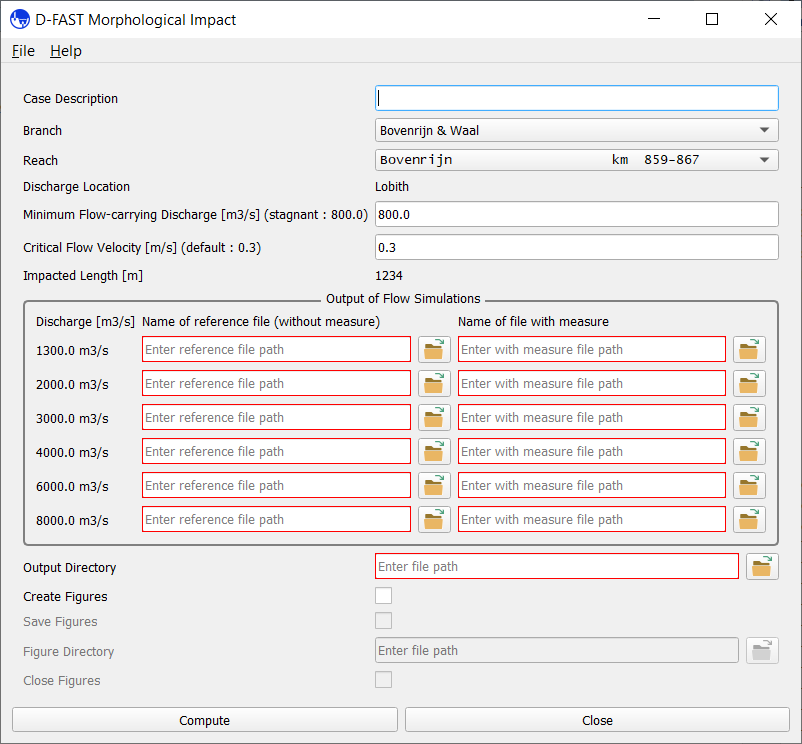
\includegraphics[width=12cm]{figures/main_dialog.png}
\caption{Example of the main dialog}
\end{figure}

The following text describes the functionality of the graphical user interface from top to bottom.
The \keyw{File} menu provides access to options to load a configuration file and to save the current selection in the gui to a configuration file.
The \keyw{Help} menu provides access to about boxes for \dfastmi itself and for the PyQt5 graphical framework.

As a user, you start specifying the branch and reach of the study.
Changing this selection will affect all fields below overwriting any previously entered values.
You have to specify the minimum flow-carrying discharge of the measure.
Together with the branch and reach selection, this determines the distance over which the river branch may be affected during the first year.
This length \unitbrackets{m} is indicated, and dynamically updated with each change you make.

Subsequently, you are presented with a list of flow conditions for which you need to provide data files representing the reference situation and the situation with the measure implemented.
The names of the files need to be specified in the edit fields below.

The last input item for the analysis is the critical flow velocity \unitbrackets{m/s} for sediment transport.
Finally, we find at the bottom of the dialog some options for the output of the \dfastmi run, and a button to run the analysis in the folder from which the program was started, and a button to end the program.

\section{Running from Python source code}
It's recommended to run \dfastmi as binary, but you may also run it directly from the Python source code.
The source code can be downloaded from \url{https://github.com/Deltares/D-FAST_Morphological_Impact}.
When using the tool for projects, please carefully check that you use the appropriate source code version.
A Python Poetry\footnote{\url{https://python-poetry.org/}} environment has been configured to relatively easily install all libraries necessary for running the tool.
See the \dfastmi Technical Reference Manual for details.
Follow the steps in the online Developer user starter guide to set up the run environment using \keyw{poetry install}.
In that case the program can be started from the command prompt as

\begin{Verbatim}
poetry run python -m dfastmi ...options...
\end{Verbatim}

or from within a running Python environment as

\begin{Verbatim}
import dfastmi.cmd
dfastmi.cmd.run()
\end{Verbatim}

where optionally the command{runmode} (default \command{GUI}), \command{configfile} (default \command{dfastmi.cfg}) and \command{rivers\_file} (default \command{Dutch\_rivers\_v2.ini}) can be specified as arguments.
\chapter{User Guidance}\label{Chp:Guidance}

\dfastmi is a rapid assessment tool that provides feedback regarding the morphological impact of river interventions on the main channel.
The tool provides first estimates based on a couple of hydrodynamic simulations.
When critical conditions are identified, this can support the call for more demanding morphological simulations.
The conceptual framework is described in \autoref{Chp:Concepts}.
This chapter starts with an overview of applications for which \dfmi is or is not suitable.
This is followed by a discussion of various assumptions and limitations of the \dfmi approach.
The steps of the analysis are subsequently described in \autoref{Chp:steps}.

\section{(Un)suitable applications}\label{Sec:SuitableApplications}

Situations in which \dfmi is commonly applied are river widening interventions outside the main channel, such as

\begin{itemize}
\item side channels
\item flood plain lowering
\item adjustment of secondary levees
\item widening of the bank region
\item adjustment of the river groynes
\end{itemize}

The tool can be used to identify potential morphological impact (both size and location) in an early stage, such as during the design phase.
Furthermore, the tool can be used to determine whether more advanced evaluation methods are required to determine whether the impact is acceptable.
\dfmi should not be used

\begin{itemize}
\item if a more advanced impact assessment method is required, typically, in case of
\begin{itemize}
\item critical conditions for shipping or river safety and/or
\item critical conditions identified by an initial \dfmi assessment and/or
\item in the final assessment of the planning phase and/or
\item if there are more strict requirements concerning quantification of the sedimentation in the context of the causation principle
\end{itemize}
\item to estimate bed level changes due to discharge extractions (e.g.~rerouting flow between the river branches would cause changes over large distances)
\item to estimate bed level changes outside the main channel
\item to estimate bed level changes due to interventions that cannot be represented well in the \dflowfm schematizations
\item to estimate bank erosion. \dfastbe should be considered instead.
\item to estimate the impact of interventions in the main channel, such as
\begin{itemize}
\item to quantify the total dredging volumes
\item to study the impact of different dredging strategies
\end{itemize}
\item to estimate bed level changes due to changes in sediment supply and/or main channel bed levels
\item to identify areas subject to erosion
\end{itemize}


\section{Assumptions and limitations}\label{Sec:Limitations}

The conceptual framework described in \autoref{Chp:Concepts} is based on a number of assumptions.
Therefore, \dfmi has some limitations regarding the application.

\begin{enumerate}
\item It's assumed that the intervention (and the subsequent morphological development) does not significantly influence the water levels.
The impact of large interventions that influence the backwater curve, may thus not be estimated accurately by \dfmi.

\item Interventions should be properly resolved on the \dflowfm mesh.
The discharges used by \dfmi should give a balanced representation of the influence of the intervention on the flow patterns.
Hence, \dfmi is not suitable for interventions that have been designed to only have a noticeable effect for flow conditions not included in the analysis.
An example of such a case is an intervention that is only active above the highest discharge level.
A conservative estimate of the possible impact of such a case can be obtained by evaluating a similar intervention for which the maximum impact on the flow field has been shifted to the highest discharge level.

\item \dfastmi is not yet suited for tidally influenced areas.
See \autoref{Sec:Tides}.

\item \label{reach_bnd} The river system is subdivided into branches and reaches.
The characteristics, such as the characteristic bed celerity and normal channel width, may vary per branch or even reach.
Interventions located across reaches, should be evaluated against the settings of the dominant reach, i.e.~the reach in which the dominant effect is to be expected (typically the reach in which the largest part of the intervention is located).
If an intervention is located close to, or even across branches, an additional verification should be done to determine whether \dfmi can be applied, and if so, how it should be applied.

\item The morphological impact of an intervention will only accumulate over the period during which the intervention is active.
The original WAQMORF algorithm selected discharges based on the specific characteristics of the intervention being evaluated, and as such it was not suited for evaluating multiple interventions at once.
The new algorithm uses a fixed set of discharges, which makes it more generic, but the reported impacted length $L_s$, i.e.~the distance over which the morphological changes can develop over the period of one year, still depends on the specified minimum flow-carrying discharge $Q_\text{thr}$, i.e.~the discharge above which the intervention will be influencing the flow.
Consider the following two interventions:

\begin{itemize}
\item One intervention that is active only at high flow (${Q_\text{thr}}_1$ is large).
Let us assume that this intervention has a significant impact on the flow patterns in the main channel at those flow conditions and hence a significant long-term morphological impact, i.e.~a large year-averaged equilibrium bed level change $\bar{\Delta z_b}_1$.
This intervention is associated with a small impacted length, ${L_s}_1 \ll {L_s}_2$, since its minimum flow-carrying discharge is exceeded only a small part of the year.
Hence, when this intervention is evaluated by itself, the \emph{first-year} impact (estimated as the equilibrium effect accumulated over the impacted length) would be modest.

\item One intervention that is almost always active (${Q_\text{thr}}_2 = 0$).
Let us assume that this intervention has very little to no morphological impact by itself, i.e.~$\bar{\Delta z_b}_2 \ll \bar{\Delta z_b}_1$.
Since this intervention is active under all flow conditions, the impacted length ${L_s}_2$ is basically equal to the distance over which any bed disturbance can travel in a year.
However, the \emph{first-year} impact of just this intervention would also be modest since $\bar{\Delta z_b}_2$ is small.
\end{itemize}

However, when the two interventions are evaluated \emph{together}, the impacted length will be based on the smaller minimum flow-carrying discharge ${Q_\text{thr}}_2$ of intervention 2 (and hence $L_s$ will be large), while the year-averaged equilibrium bed level change of the two interventions together will be similar to that of the first intervention, $\bar{\Delta z_b}_1$.
The estimated first-year effect, obtained by integrating $\bar{\Delta z_b}_1$ over ${L_s}_2$, will be significantly bigger than each of the measures individually.
We conclude that it's wise to only evaluate interventions together if they have similar threshold discharges.
If the threshold discharges differ significantly, then the estimate for the first-year effect will be on the conservative side.

\item When combining multiple interventions, or when making a single intervention longer, you will reach the point at which the effect of an intervention on the flow can no longer be seen as one stretch where water leaves the main channel, and one where it flows back to it (or the other way around).
There will be multiple of these stretches due to the sequence of interventions, or due to the alongstream variation of the left and right floodplain width.
As a result, the morphological impact will not be represented by a single sedimentation (or erosion) area, but a series of them.
Earlier versions, therefore, suggested to restrict the use of this tool to interventions shorter than 4 km, but this restriction can be relaxed by not only taking into account the most upstream area in the estimation of the first-year sedimentation volume, but all separate areas.
See \autoref{Sec:DredgeVol}.
However, it's still preferred to evaluate interventions less than the length of one flood plain section.

\item \dfastmi doesn't use any information about the bed composition.
It doesn't get information about non-erodible layers, nor about natural variability in the erodibility of the bed material.
As such, it is more difficult for \dfmi to predict scour accurately than sedimentation.
The primary purpose of \dfmi is the estimation of sedimentation that may cause problems for navigation.
As such, it is better suited for evaluating interventions that increase the flow area than interventions that decrease the flow area.

\item \dfastmi conceptual model is based on a change in the discharge in the main channel.
Such a change may be caused by changes in the floodplain, or changes in the main channel.
When the intervention affects the floodplain, its impact on the main channel is easy to interpret since both simulations with and without the intervention use the same bed levels for that area.
However, when the intervention affects the main channel, for instance by deepening, the resulting impact (sedimentation to get back to the original bed level) must be interpreted as relative to the bed levels of the simulation \emph{with} the intervention implemented.
Furthermore, it should be noted that \autoref{Eq:zbEqui} is evaluated using the water depth $h$ obtained from the reference simulation.
If the intervention includes a significant change to the bed level in the main channel, this approximation may no longer be valid.
Therefore, \dfmi is not recommended for such interventions.

\item \dfastmi does not take into account the dynamic feedback that morphological change may have on the hydrodynamics.
This general limitation is related to the following three statements.

\item \dfastmi assumes that a new equilibrium can be reached by adjusting the bed level locally such that the flow velocity at that point returns to the original value.
This is the result of the 1D conceptual approach in which the flow cannot redistribute laterally.
Consequently, \dfmi is better at estimating the one-dimensional, width-averaged impact than the two-dimensional, lateral variability of the impact.
The lateral variability may force further variability up- and downstream that will not be identified by \dfmi.

\item \dfastmi focuses on the long-term equilibrium effect and the rate of change.
It does not estimate in any way the dynamic effect of the intervention: the erosion wave downstream of a sedimentation area caused by an increase in flow area, or the sedimentation wave downstream of an erosion area.
These dynamic effects will be of the same order as the first-year sedimentation or erosion, but of opposite sign.
They will propagate downstream unless they are compensated by dredging or suppletion once.

\item \dfastmi does not take into account bank erosion or bank failure due to erosion; neither related to the dynamic effect mentioned in the previous bullet, nor related to the long-term change to the bed levels.
Consider using \dfastbe, or expert judgment.

\end{enumerate}

\chapter{Conceptual framework}

This chapter describes the conceptual framework of the method used by \dfastmi and the derivation of the river parameters used for the Dutch rivers.

\section{Characteristics of bed level changes due to river measures}

A river measure, i.e.~a local river adjustment (typically a flow capacity enlarging adjustment) outside the main channel, may result in changes in the flow pattern within the main channel.
The bed levels within the main channel will react to such changes depending on the

\hspace{1cm}\emph{magnitude, duration and length scale of these flow pattern changes in the main channel.}

Hence, the core focus of the rule-of-thumb is to determine and characterize the changes in the flow pattern within the main channel.
Here, we define the main channel as the part of the river between the groyne heads.

At the upstream end of the floodplain adjustment part of the main channel discharge will leave the main channel, which will flow through the enlarged floodplain, secondary channel or bank area, and return to the main channel at the downstream end of the project area.
The resulting changes in the main channel flow pattern cause sedimentation in the main channel at the upstream "offtake" of the new outflow and erosion at the downstream "confluence" when the flow enters the main channel again.
Because the river discharge varies, the pattern will also vary during the year
As a result a part of the main channel bed level adjustment is stationary and a part of the adjustment is transitional and it will migrate downstream.
A reduction in the water depth may thus not only be observed locally where the flow diverges into the flood plain, but also downstream thereof.

The bed level change due to river enlargement can largely be characterized as follows

\begin{itemize}
\item The magnitude of the bed level change varies over the seasons; the maximum change is observed at the end of the flood season and the adjustment reaches a minimum at the end of the low flow period.

\item Local evaluation of the bed level changes is insufficient because of partial downstream migration of the bed level changes.

\item The maximum impact is observed on that side of the river which is closest to the adjustment.
\end{itemize}

Because part of the bed level changes migrate downstream, the morphological impact on projects located downstream may be increased.
After all, the maximum bed level change of one single river enlarging measure is reached at the end of the flood period and it's the result of that flood period.
However, when a series of measures along the river are combined (for instance, lowering of the groynes along a reach) the downstream bed level changes may be increased by accumulation of downstream migrating bed waves, such that the accumulated bed level change may be significantly larger.
In other words, river measures extending over longer reaches may result in a larger morphodynamic response than comparable but more isolated measures.

The aforementioned observations result in the following premisses.
The rule-of-thumb described in the following sections

\begin{itemize}
\item will only be valid for the estimation of the impact of local measures with a length of at most one flood plain,

\item should take into account seasonal variations, and

\item needs to be estimate the spatial pattern of the bed level change.
\end{itemize}


\section{Characterization of the changes in the main channel flow pattern}

When a measure in the floodplains does not include something like a permanently active secondary channel, the flow pattern in the main channel will only be affected during flood conditions.
If on the other hand, such a secondary channel (or other measure active under medium to low flow conditions such as groyne adjustments) is included in the design then the flow pattern will also be influenced during transitional or even low flow conditions.
It's therefore critical to determine the effect of the measure on the main channel flow pattern at different discharge levels.

Secondary channels may have a major impact on the morphodynamics of the main channel.
The magnitude of the discharge through the secondary channel varies as function of the river discharge.
Because the hydraulic conditions of the secondary channel can change over time (e.g.~due to vegetation, siltation, or erosion) the discharge through a secondary channel is typically controlled by some hydraulic structure.
The typical characteristics of a weir (overlaat, drempel) and orifice (onderlaat, duiker) are shown in \autoref{Fig1}.

\begin{figure}
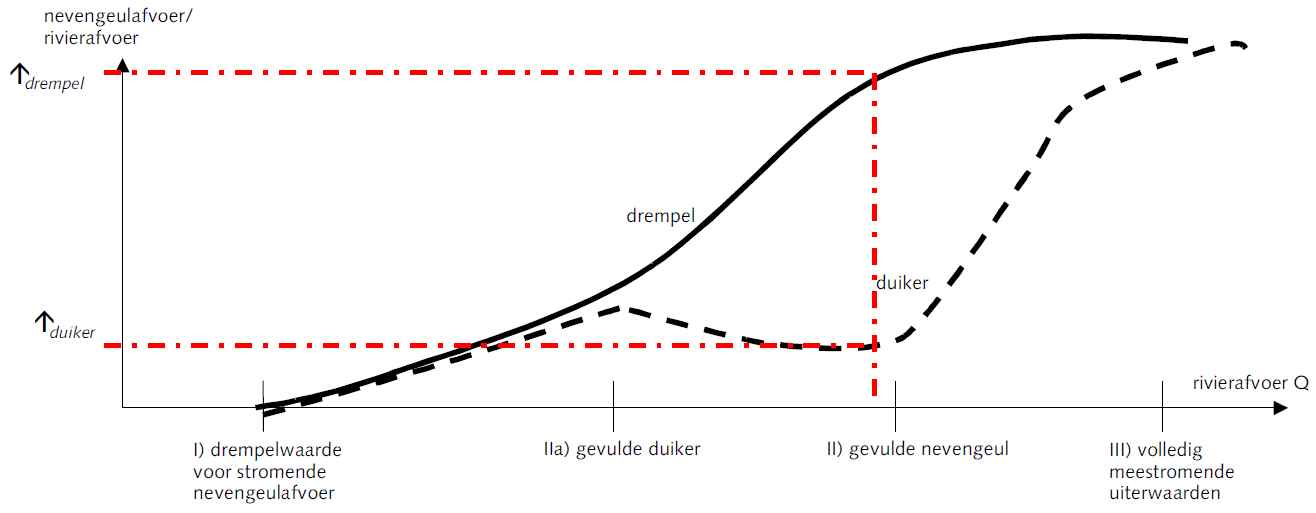
\includegraphics[width=\columnwidth]{figures/Fig1.png}
\caption{Schematic of the controlled discharge through a secondary channel.}
\label{Fig1}
\end{figure}

The discharge through a secondary channel is characterized by a number of special conditions as illustrated by \autoref{Fig1}:

\begin{enumerate}
\item the beginning of flow through the secondary channel
\item the bankfull secondary channel
\item the fully developed flow in the secondary channel and surrounding floodplain.
\end{enumerate}

When the discharge through the secondary channel is controlled by an orifice, the fully flooded condition may add an additional characteristic discharge.

In order to characterize the flow patterns during flood it's necessary to distinguish the condition in which the flood plains just start to carry flows, and the condition of fully developed flow in the flood plains.
Based on results of 1D simulations shown in \autoref{Fig2a} it has been concluded that for the Rhine branches a discharge of 6000 m\textsuperscript{3}/s at Lobith can be used as the boundary between those two conditions.
The flow through the bank zone (\autoref{Fig2b}) is also largely developed for discharges at Lobith larger than
6000 m\textsuperscript{3}/s.

\begin{figure}
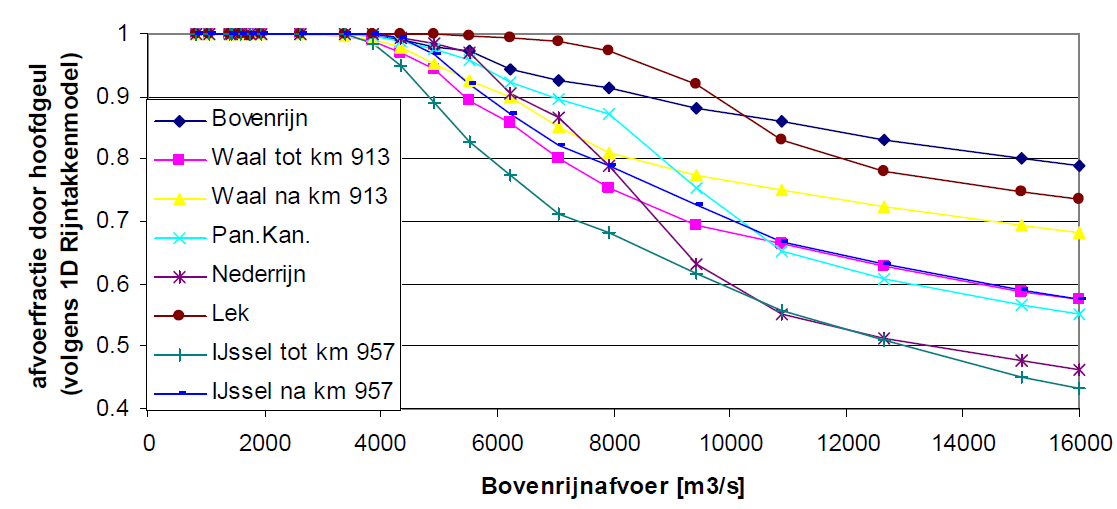
\includegraphics[width=\columnwidth]{figures/Fig2a.png}
\caption{Reach-averaged discharge fraction through the main channel (based on 1D model of the Rhine branches).}
\label{Fig2a}
\end{figure}

\begin{figure}
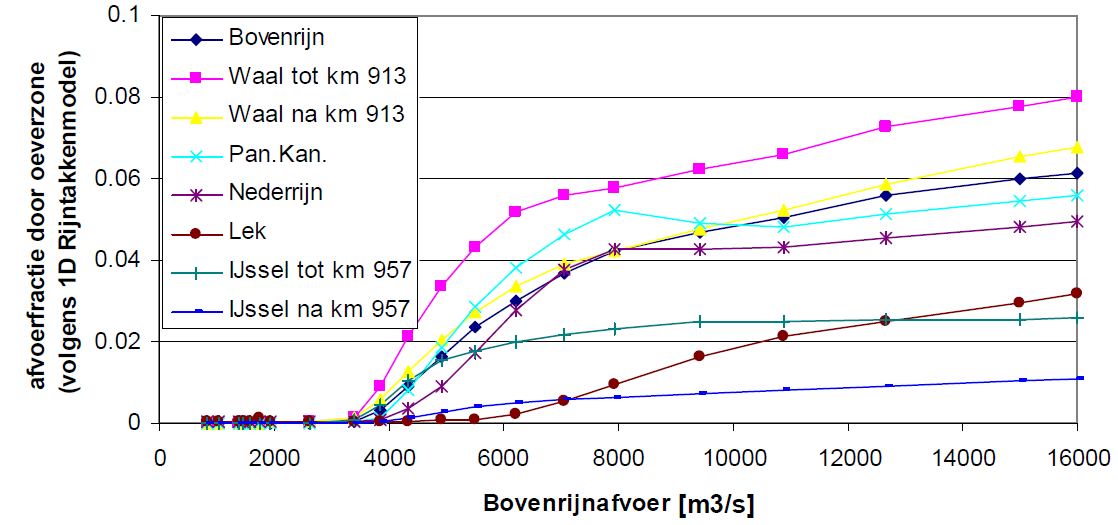
\includegraphics[width=\columnwidth]{figures/Fig2b.png}
\caption{Reach-averaged discharge fraction through the bank zone (based on 1D model of the Rhine branches).}
\label{Fig2b}
\end{figure}

These characteristic discharge values can be used to schematize the river hydrograph effectively by means of a limited number of discrete discharge conditions.
Three discharge blocks turn out to be sufficient for many measures as may bed concluded from \autoref{Tab1}.
That is why it has been concluded that \emph{three flow conditions are sufficient to schematize the yearly hydrograph for the purpose of estimating the morphological impact of local measures}.

\begin{table}
\small
%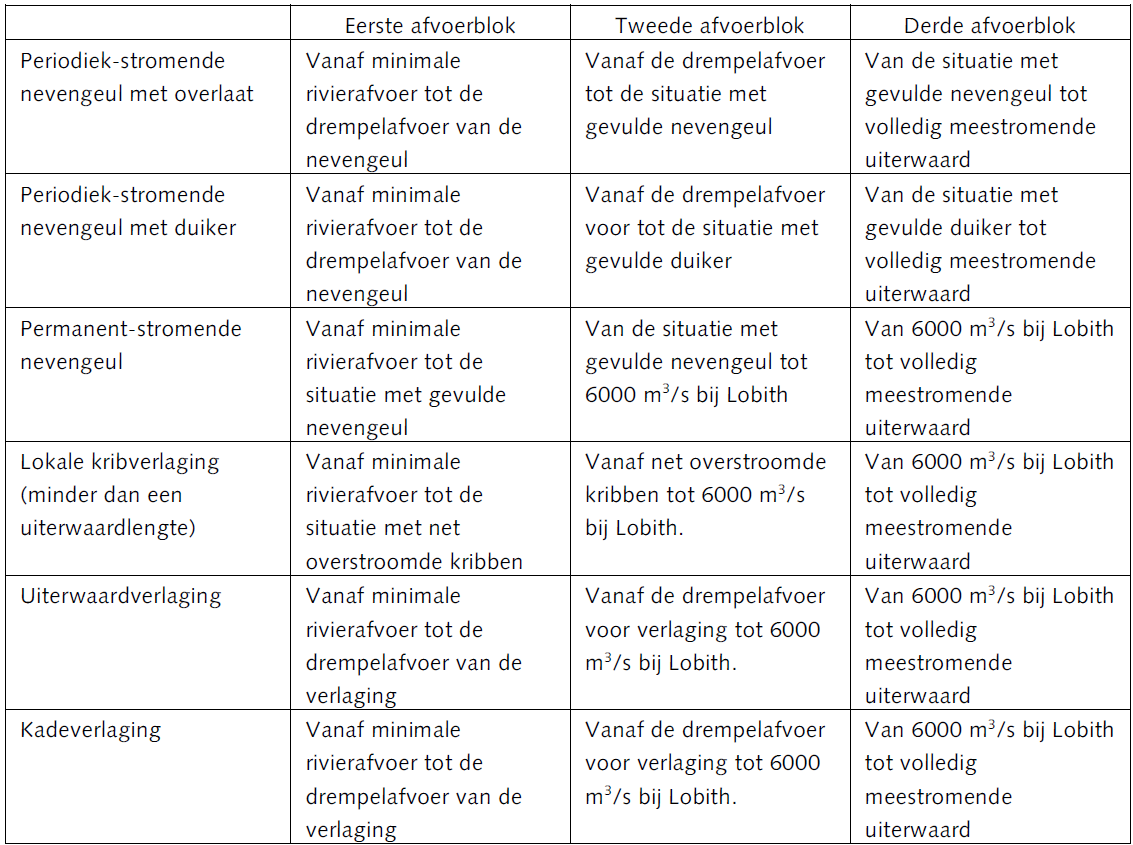
\includegraphics[width=\columnwidth]{figures/Tab1a.png}
\begin{tabular}{p{\columnwidth/4-12pt}|p{\columnwidth/4-12pt}|p{\columnwidth/4-12pt}|p{\columnwidth/4-12pt}}
 & first block & second block & third block \\ \hline
periodically flowing secondary channel with weir & from minimum river flow to minimum discharge for secondary channel & from minimum discharge for secondary channel to bankfull secondary channel & from bankfull secondary channel to fully developed flood plain flow \\ \hline
periodically flowing secondary channel with orifice & from minimum river flow to minimum discharge for secondary channel & from minimum discharge for secondary channel to fully flooded orifice & from fully flooded orifice to fully developed flood plain flow \\ \hline
permanently flowing secondary channel & from minimum river flow to bankfull secondary channel & from bankfull secondary channel to 6000 m\textsuperscript{3}/s at Lobith & from 6000 m\textsuperscript{3}/s at Lobith to fully developed flood plain flow \\ \hline
local lowering of groynes (less than flood plain length) & from minimum river flow to flooded groynes & from flooded groynes to 6000 m\textsuperscript{3}/s at Lobith & from 6000 m\textsuperscript{3}/s at Lobith to fully developed flood plain flow \\ \hline
lowering of the flood plain & from minimum river flow to minimum discharge for new flood plain threshold & from new flood plain threshold to 6000 m\textsuperscript{3}/s at Lobith & from 6000 m\textsuperscript{3}/s at Lobith to fully developed flood plain flow \\ \hline
lowering of levees & from minimum river flow to minimum discharge for new levee threshold & from new levee threshold to 6000 m\textsuperscript{3}/s at Lobith & from 6000 m\textsuperscript{3}/s at Lobith to fully developed flood plain flow \\
\end{tabular}

\caption{Overview of discharge conditions for various measures in a free flowing Rhine branch.}
\label{Tab1}
\end{table}

For a river reach in which water levels (and hence flow conditions) are controlled by means of barriers for a period $T_\text{stuw}$, the minimum river discharge is determined by the river discharge at which the barriers are opened.
\autoref{Fig6} shows that the barriers in the Nederrijn are opened at a discharge of 1500 m\textsuperscript{3}/s in the Bovenrijn at Lobith (this value is exceeded during 57 \% of the year) and that the branch is approximately free flowing for discharges above 2200 m\textsuperscript{3}/s in the Bovenrijn at Lobith (exceeded during 33 \% of the year).

\begin{table}
%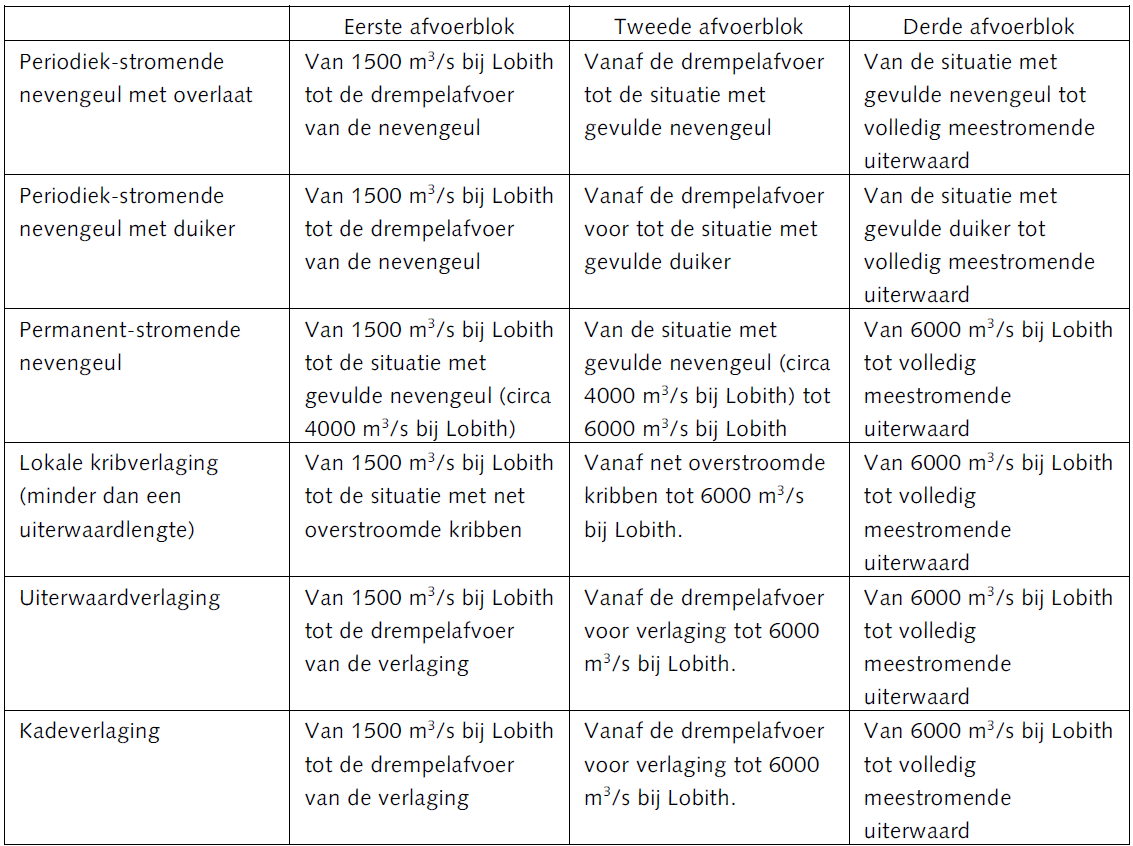
\includegraphics[width=\columnwidth]{figures/Tab1b.png}
\begin{tabular}{p{\columnwidth/4-12pt}|p{\columnwidth/4-12pt}|p{\columnwidth/4-12pt}|p{\columnwidth/4-12pt}}
 & first block & second block & third block \\ \hline
periodically flowing secondary channel with weir & from 1500 m\textsuperscript{3}/s at Lobith to minimum discharge for secondary channel & from minimum discharge for secondary channel to bankfull secondary channel & from bankfull secondary channel to fully developed flood plain flow \\ \hline
periodically flowing secondary channel with orifice & from 1500 m\textsuperscript{3}/s at Lobith to minimum discharge for secondary channel & from minimum discharge for secondary channel to fully flooded orifice & from fully flooded orifice to fully developed flood plain flow \\ \hline
permanently flowing secondary channel & from 1500 m\textsuperscript{3}/s at Lobith to bankfull secondary channel (about 4000 m\textsuperscript{3}/s at Lobith) & from bankfull secondary channel (about 4000 m\textsuperscript{3}/s at Lobith) to 6000 m\textsuperscript{3}/s at Lobith & from 6000 m\textsuperscript{3}/s at Lobith to fully developed flood plain flow \\ \hline
local lowering of groynes (less than flood plain length) & from 1500 m\textsuperscript{3}/s at Lobith to flooded groynes & from flooded groynes to 6000 m\textsuperscript{3}/s at Lobith & from 6000 m\textsuperscript{3}/s at Lobith to fully developed flood plain flow \\ \hline
lowering of the flood plain & from 1500 m\textsuperscript{3}/s at Lobith to minimum discharge for new flood plain threshold & from new flood plain threshold to 6000 m\textsuperscript{3}/s at Lobith & from 6000 m\textsuperscript{3}/s at Lobith to fully developed flood plain flow \\ \hline
lowering of levees & from 1500 m\textsuperscript{3}/s at Lobith to minimum discharge for new levee threshold & from new levee threshold to 6000 m\textsuperscript{3}/s at Lobith & from 6000 m\textsuperscript{3}/s at Lobith to fully developed flood plain flow \\
\end{tabular}

\caption{Overview of discharge conditions for various measures along the Nederrijn.}
\label{Tab2}
\end{table}

\begin{table}
%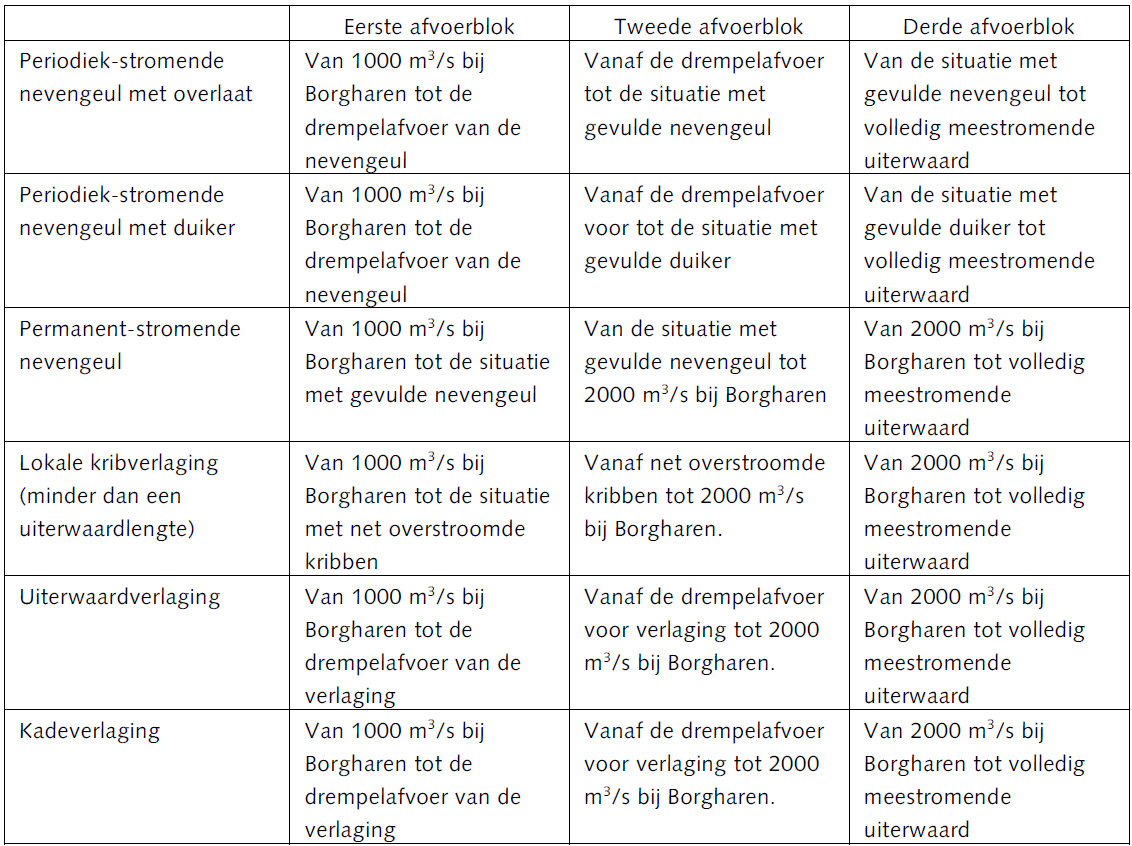
\includegraphics[width=\columnwidth]{figures/Tab1c.png}
\begin{tabular}{p{\columnwidth/4-12pt}|p{\columnwidth/4-12pt}|p{\columnwidth/4-12pt}|p{\columnwidth/4-12pt}}
 & first block & second block & third block \\ \hline
periodically flowing secondary channel with weir & from 1000 m\textsuperscript{3}/s at Borgharen to minimum discharge for secondary channel & from minimum discharge for secondary channel to bankfull secondary channel & from bankfull secondary channel to fully developed flood plain flow \\ \hline
periodically flowing secondary channel with orifice & from 1000 m\textsuperscript{3}/s at Borgharen to minimum discharge for secondary channel & from minimum discharge for secondary channel to fully flooded orifice & from fully flooded orifice to fully developed flood plain flow \\ \hline
permanently flowing secondary channel & from 1000 m\textsuperscript{3}/s at Borgharen to bankfull secondary channel & from bankfull secondary channel to 2000 m\textsuperscript{3}/s at Borgharen & from 2000 m\textsuperscript{3}/s at Borgharen to fully developed flood plain flow \\ \hline
local lowering of groynes (less than flood plain length) & from 1000 m\textsuperscript{3}/s at Borgharen to flooded groynes & from flooded groynes to 2000 m\textsuperscript{3}/s at Borgharen & from 2000 m\textsuperscript{3}/s at Borgharen to fully developed flood plain flow \\ \hline
lowering of the flood plain & from 1000 m\textsuperscript{3}/s at Borgharen to minimum discharge for new flood plain threshold & from new flood plain threshold to 2000 m\textsuperscript{3}/s at Borgharen & from 2000 m\textsuperscript{3}/s at Borgharen to fully developed flood plain flow \\ \hline
lowering of levees & from 1000 m\textsuperscript{3}/s at Borgharen to minimum discharge for new levee threshold & from new levee threshold to 2000 m\textsuperscript{3}/s at Borgharen & from 2000 m\textsuperscript{3}/s at Borgharen to fully developed flood plain flow \\
\end{tabular}

\caption{Overview of discharge conditions for various measures along the Meuse.}
\label{Tab3}
\end{table}

\begin{figure}
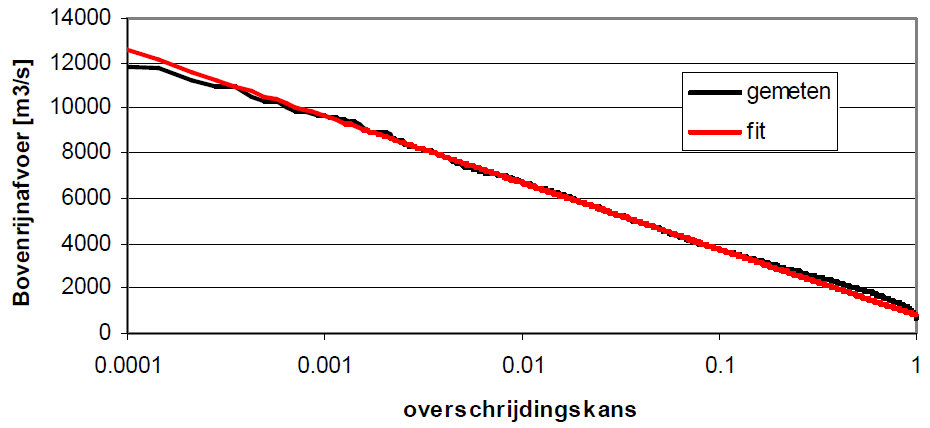
\includegraphics[width=\columnwidth]{figures/Fig3a.png}
\caption{Discharge exceedance curve for the Bovenrijn at Lobith (1970-2000).}
\label{Fig3a}
\end{figure}

\begin{figure}
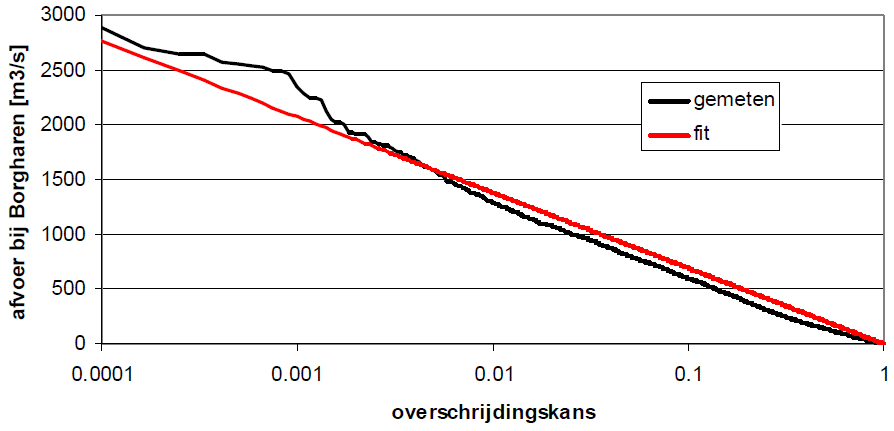
\includegraphics[width=\columnwidth]{figures/Fig3b.png}
\caption{Discharge exceedance curve for the Meuse at Borgharen (1975-2007).}
\label{Fig3b}
\end{figure}

In order to quickly estimate the yearly exceedance period for a given discharge, the discharge exceedance curve for the Bovenrijn has been approximated by a curve fitted through the observational data for the period 1970-2000 (\autoref{Fig3a}).
The number of days that the discharge $Q_\text{Bovenrijn}$ in the Bovenrijn at lobith is exceeded is given by

\begin{equation}
\label{Eq1a}
T_\text{exceedance, Bovenrijn} = 365 e^{\left ( \frac{800 -  Q_\text{Bovenrijn}}{1280} \right )}
\end{equation}

For the Meuse, in which --- due to imbrication (Grensmaas) and barriers (Zandmaas) --- the higher discharges are more important for the morphological development, the exceedance period for discharges at Borgharen can be estimated as

\begin{equation}
\label{Eq1b}
T_\text{exceedance, Meuse} = 365 e^{\left ( \frac{-  Q_\text{Borgharen}}{300} \right )}
\end{equation}

\section{Scientific background of the relaxation model for morphological change}

The rule-of-thumb used to determine the first estimate of the morphological effects within the main channel is based on a highly simplified model of the morphodynamics.
That model and the resulting rule-of-thumb are described in this section.

We start by assuming a quasi-stationary flow pattern and an outflow of discharge and sediment from the main channel while the local water level is independent of the hydraulic and morphological changes in the main channel (a \emph{rigid-lid} approximation).

\begin{figure}
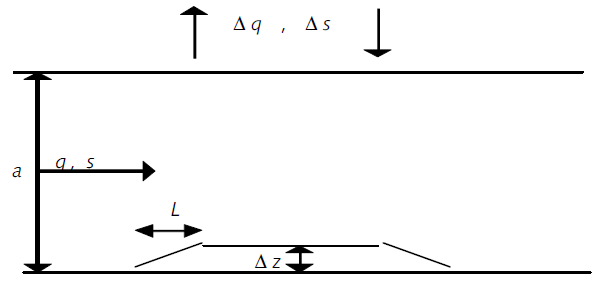
\includegraphics[width=\columnwidth]{figures/Fig4.png}
\caption{Schematic representation of the outflow of water and sediment}
\label{Fig4}
\end{figure}

The response of the main channel is represented here by a bed level change $\Delta z_b$ \unitbrackets{m} (raise or lowering) which is small relative to the local water depth.
The mass balance of the water and the sediment in the main channel can be written as
%
\begin{align}
&\text{water} & \pdiff{q_\text{mc}}{s} = -q_\text{out} \label{Eq2} \\
&\text{sediment} & \pdiff{z_b}{t} + \pdiff{s_\text{mc}}{s} = -s_\text{out} \label{Eq3}
\end{align}
%
in which
%
\begin{symbollist}
\item[$q_\text{mc}$] main channel unit discharge \unitbrackets{m\textsuperscript{2}/s}
\item[$q_\text{out}$] \emph{outflow of} unit discharge \emph{to} the flood plain per unit length \unitbrackets{m\textsuperscript{2}/sm}
\item[$s$] streamwise coordinate \unitbrackets{m}
\item[$z_b$] bed level change due to measure \unitbrackets{m}
\item[$s_\text{mc}$] main channel unit sediment transport including pores \unitbrackets{m\textsuperscript{2}/s}
\item[$s_\text{out}$] \emph{outflow of} unit sediment transport including pores \emph{to} the flood plain per unit length \unitbrackets{m\textsuperscript{2}/sm}
\end{symbollist}

Note that the outflow of sediment is assumed to be a consequence of the outflow of discharge only; the conceptual framework does not allow for selective removal of only sediments.	
The unit sediment transport capacity in the main channel, $s_\text{mc}$, is approximated by $s_\text{mc} = m \left ( q_\text{mc} / h \right )^b$ with $h$ the water depth \unitbrackets{m} in the main channel, $m$ a dimensionless calibration factor and a dimensionless sediment transport exponent $b$ about 5 \citep{Engelundh67}.
Using this approximation the gradients in the sediment transport capacity can be written as
%
\begin{align}
\pdiff{s_\text{mc}}{s} &= m b \left ( \frac{q_\text{mc}}{h} \right )^{b-1} \pdiff{(q_\text{mc} / h)}{s} \\
&= m b \left ( \frac{q_\text{mc}}{h} \right )^{b-1} \left [ \frac{1}{h} \pdiff{q_\text{mc}}{s} - \frac{q_\text{mc}}{h^2} \pdiff{h}{s} \right ] \\
&= b \frac{s_\text{mc}}{q_\text{mc}} \pdiff{q_\text{mc}}{s} - b \frac{s_\text{mc}}{h} \pdiff{h}{s} \\
&\approx b \frac{s_\text{mc}}{q_\text{mc}} \pdiff{q_\text{mc}}{s} + b \frac{s_\text{mc}}{h} \pdiff{z_b}{s}
\label{Eq4}
\end{align}
%
if we assume that the water level gradient is negligible ($\pdiff{z_w}{s} \approx 0$) such that $\pdiff{h}{s} \approx -\pdiff{z_b}{s}$.
Substitution of \autoref{Eq4} into \autoref{Eq3} gives
%
\begin{equation}
\pdiff{z_b}{t} + b \frac{s_\text{mc}}{q_\text{mc}} \pdiff{q_\text{mc}}{s} + b \frac{s_\text{mc}}{h} \pdiff{z_b}{s} = -s_\text{out}
\label{Eq5a}
\end{equation}
%
which after substitution of \autoref{Eq2} in the second term becomes
%
\begin{equation}
\frac{h}{b s_\text{mc}} \pdiff{z_b}{t} + \pdiff{z_b}{s} = h \frac{q_\text{out}}{q_\text{mc}} - h \frac{s_\text{out}}{b s_\text{mc}}
\label{Eq5}
\end{equation}

The dynamic bed level changes will develop starting from the upstream end of the measure.
The length $L$ over which this sedimentation occurs (i.e.~varies from 0 upstream to maximum amount $\Delta z_b$ downstream) corresponds to the reach over which discharge leaves the main channel and in which the flow pattern is adjusted by the reduced discharge as sketched in \autoref{Fig4}.
Hence, this length $L$ may thus be significantly shorter than the length of the measure or the distance between the inflow and outflow openings of a secondary channel.
The integration of \autoref{Eq5} over this length $L$ results in a relaxation model for the dynamic bed level change due to the measure
%
\begin{equation}
\frac{h}{b s_\text{mc}} \int_0^L \pdiff{z_b}{t} ds + \int_0^L \pdiff{z_b}{s} ds = \int_0^L \left [ h \frac{q_\text{out}}{q_\text{mc}} - h \frac{s_\text{out}}{b s_\text{mc}} \right ] ds
\label{Eq5a}
\end{equation}
%
\begin{equation}
\frac{h}{b s_\text{mc}} L^* \pdiff{\Delta z_b}{t} + \Delta z_b = - h \frac{\Delta q_\text{mc}}{q_\text{mc}} + h \frac{\Delta s_\text{mc}}{b s_\text{mc}}
\label{Eq5b}
\end{equation}
%
which $\Delta q_\text{mc}$ is the total change in unit discharge in the main channel due to the measure \unitbrackets{m\textsuperscript{2}/s} and $\Delta s_\text{mc}$ is the total change in unit sediment transport due to the measure \unitbrackets{m\textsuperscript{2}/s}.
Please note that $q_\text{out}$ was defined above positive for fluxes towards the flood plain, however, the resulting change $\Delta q_\text{mc}$ in the unit discharge within the main channel will be negative for such conditions (equivalently for $s_\text{out}$ and $\Delta s_\text{mc}$); this introduces a sign change on the right hand side.
%
\begin{equation}
\diff{\Delta z_b}{t} = \frac{\Delta z_{b,\text{eq}} - \Delta z_b}{T_m}
\label{Eq5dif}
\end{equation}
%
with a morphological time scale \unitbrackets{s}
%
\begin{equation}
T_m \approx \frac{h L}{b s_\text{mc}}
\label{Eq5T}
\end{equation}
%
and an equilibrium bed level change \unitbrackets{m} given by
%
\begin{equation}
\Delta z_{b,\text{eq}} = -h \left ( \frac{\Delta q_\text{mc}}{q_\text{mc}} - \frac{\Delta s_\text{mc}}{b s_\text{mc}} \right )
\label{Eq6}
\end{equation}
%
This relaxation behaviour can also be observed in the results of the numerical models (both 1D and 2D).

The rule-of-thumb is derived by posing that the bed level change $\Delta z_b$ can be interpreted as the bed level change due to a measure over a distance $L$ along a stream line starting from the upstream end of the measure.
The equilibrium value $\Delta z_{b,\text{eq}}$ depends according \autoref{Eq6} on the (original) water depth, the relative change in unit discharge and the relative change in the sediment transport.
The latter term is the result of the sediment flux into the secondary channel which dampens the effect of reduced sediment transport capacity in the main channel.
Ignoring this relatively minor dampening term results in a more conservative estimate.
For measures over a short distance (i.e.~for the type of measures for which the rule-of-thumb is applicable) the water level changes are an order of magnitude smaller than the bed level changes.
Therefore, one can rewrite \autoref{Eq6} to state that the equilibrium bed level change $\Delta z_{b,\text{eq}}$ equals the product of the water depth and the relative change in the main channel velocity $u$ \unitbrackets{m/s}:
%
\begin{equation}
\Delta z_{b,\text{eq}} \approx -h \left ( \frac{\Delta u}{u} \right )
\label{Eq6v2}
\end{equation}
%
A similar result can be obtained for graded bed material (sand/gravel mixtures) if it's assumed that the individual sediment fractions don't influence each other's mobility (Appendix C in \citet{Waterdienst2008}).
Such an assumption is valid at sufficiently high bed shear stresses, such as during flood conditions.

\section{The relaxation model applied to seasonal variability}

The bed level development during a relaxation period is (as a solution of \autoref{Eq5dif}) given by
%
\begin{equation}
z_{b,i} = z_{b,i} (0) + [z_{b,i,\text{eq}} - z_{b,i}(0)](1 - e^{-t/T_{m,i}})
\label{Eq7}
\end{equation}
%
with
%
\begin{symbollist}
\item[$z_{b,i}$] \unitbrackets{m} the morphological effect of the measure during period $i$
\item[$z_{b,i}(0)$] \unitbrackets{m} the morphological effect at the start of period $i$
\item[$z_{b,i,\text{eq}}$] \unitbrackets{m} the equilibrium effect of the measure during period $i$
\item[$t$] \unitbrackets{day} time
\item[$T_{m,i}$] \unitbrackets{day} the morphological time scale during period $i$
\end{symbollist}

\begin{figure}
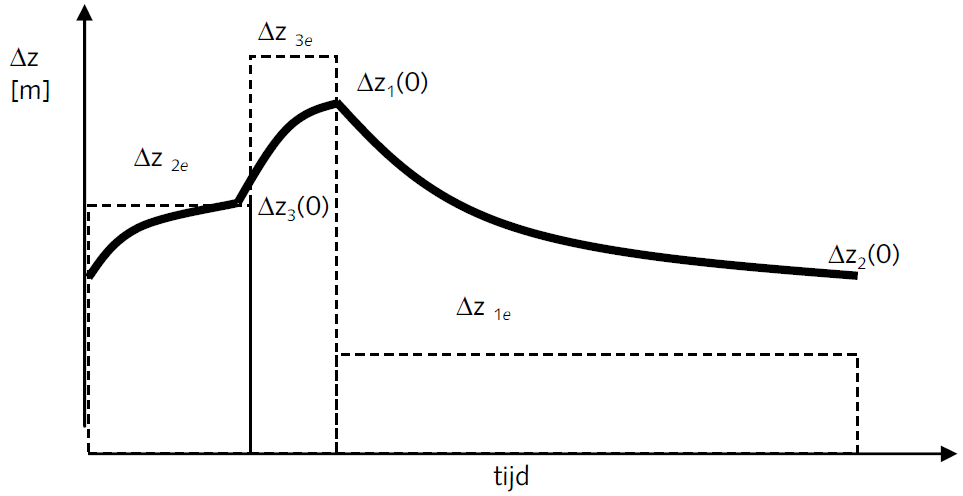
\includegraphics[width=\columnwidth]{figures/Fig5.png}
\caption{Schematic maximum bed level changes at the upstream end.}
\label{Fig5}
\end{figure}

\autoref{Eq7} implies that at the end of period $i$ (lasting for a period of $T_i$ days) the morphological effect of the measure is given by
%
\begin{equation}
z_{b,i+1}(0) = z_{b,i} (0) \sigma_i + z_{b,i,\text{eq}} (1-\sigma_i) \text{ with } \sigma_i = e^{-T_i/T_{m,i}}
\label{Eq8a}
\end{equation}

If the yearly hydrograph is schematized using three periods, one obtains the following set of three equations for the three periods by assuming periodicity (the final bed level of the third period equals the initial bed level of the first period)
%
\begin{align}
z_{b,2}(0) &= z_{b,1}(0) \sigma_1 + z_{b,1,\text{eq}} (1-\sigma_1) \label{Eq8b} \\
z_{b,3}(0) &= z_{b,2}(0) \sigma_2 + z_{b,2,\text{eq}} (1-\sigma_2) \label{Eq8c} \\
z_{b,1}(0) &= z_{b,3}(0) \sigma_3 + z_{b,3,\text{eq}} (1-\sigma_3) \label{Eq8d}
\end{align}

We can solve these three equations for the unknown bed levels $z_{b,1}(0)$, $z_{b,2}(0)$ and $z_{b,3}(0)$.
This gives the following three expressions
%
\begin{align}
z_{b,1}(0) &= \frac{z_{b,1,\text{eq}} (1-\sigma_1) \sigma_2 \sigma_3 + z_{b,2,\text{eq}} (1-\sigma_2) \sigma_3 + z_{b,3,\text{eq}} (1-\sigma_3)}{1 - \sigma_1 \sigma_2 \sigma_3} \label{Eq8e} \\
z_{b,2}(0) &= \frac{z_{b,1,\text{eq}} (1-\sigma_1) + z_{b,2,\text{eq}} (1-\sigma_2) \sigma_3 \sigma_1 + z_{b,3,\text{eq}} (1-\sigma_3) \sigma_1}{1 - \sigma_1 \sigma_2 \sigma_3} \label{Eq8f} \\
z_{b,3}(0) &= \frac{z_{b,1,\text{eq}} (1-\sigma_1) \sigma_2 + z_{b,2,\text{eq}} (1-\sigma_2) + z_{b,3,\text{eq}} (1-\sigma_3) \sigma_1 \sigma_2}{1 - \sigma_1 \sigma_2 \sigma_3} \label{Eq8g}
\end{align}

The lower bound for the morphological impact of the measure will be equal to $\min[z_{b,1}(0), z_{b,2}(0), z_{b,3}(0)]$ and the upper bound is given by $\max[z_{b,1}(0), z_{b,2}(0), z_{b,3}(0)]$.
For the schematized hydrograph shown in \autoref{Fig5} the bed level change is

\begin{itemize}
\item maximum at $z_{b,1}(0)$ (\autoref{Eq8e}) after flood period 3 (the third block in \autoref{Tab2})
\item minimum at $z_{b,2}(0)$ (\autoref{Eq8f}) after the low flow period 1 (the first block in \autoref{Tab2}).
\end{itemize}

In case the river section is experiences nearly stagnant flow conditions due to barriers a yearly period without bed level changes is inserted between low flow period 1 and the transitional flow period 2.\footnote{Earlier versions of this manual suggested that this period might be inserted between the flood period 3 and the low flow period 1, but algorithmically it was always placed between periods 1 and 2.}

We can't only obtain expressions for the two extreme (minimum, maximum) values but we can also determine an expression for the year-averaged bed level change by integrating \autoref{Eq7} per constant discharge period to
%
\begin{align}
\bar{z}_{b,i} &= \frac{1}{T_i} \int_0^{T_i}{z_{b,i} (0) + [z_{b,i,\text{eq}} - z_{b,i}(0)](1 - e^{-t/T_{m,i}})}dt \\
&= \frac{1}{T_i} \left . \left ( {z_{b,i,\text{eq}} t + [z_{b,i,\text{eq}} - z_{b,i}(0)]T_{m,i} e^{-t/T_{m,i}}} \right ) \right |_{t=0}^{t=T_i} \\
&= z_{b,i,\text{eq}} + [z_{b,i,\text{eq}} - z_{b,i}(0)] \frac{T_{m,i}}{T_i} ( e^{-T_i/T_{m,i}} - 1 )
\end{align}
%
and over all periods to
%
\begin{equation}
\bar{z}_b = \frac{\sum{z_{b,i,\text{eq}} T_i}}{\sum{T_i}} + \frac{\sum{(z_{b,i,\text{eq}}-z_{b,i}(0)) T_{m,i} (\sigma_i-1)}}{\sum{T_i}}
\label{Eq8h}
\end{equation}
%
If all bed level changes are removed after the flood period by means of dredging, the yearly dredging amount can finally be estimated by ignoring any excess depth.
After all, the maximum bed level change at the end of the flood season can with $z_{b,1}(0) = 0$ and \autoref{Eq8a} to \autoref{Eq8i} be expressed as the maximum dredging depth $z_\text{mdd}$

\begin{equation}
z_\text{mdd} = z_{b,1,\text{eq}}(1-\sigma_1) \sigma_2 \sigma_3 + z_{b,2,\text{eq}} (1-\sigma_2) \sigma_3 + z_{b,3,\text{eq}} (1-\sigma_3)
\label{Eq8i}
\end{equation}

Because this estimated doesn't take into account the sediment supply by the river, \autoref{Eq8i} can overestimate the maintenance dredging required.
\autoref{Eq8i} is therefore not included in the \dfastmi analysis.

\section{Estimate of the spatial distribution of the bed level changes}

\autoref{Eq8e} gives the maximum and \autoref{Eq8f} gives the minimum bed level change at the upstream end of the measure.
Moving downstream for that point, the bed level change consists of a minimum bed level change $z_{b,1,\text{eq}}$ plus the part of the flood deposit that moves downstream during low flow conditions.
During a flood the downstream migrating sedimentation volume may temporarily even cause bed level changes larger than $z_{b,2,\text{eq}}$ but this is rather unlikely.
For convenience, it's therefore assumed that the maximum and minimum bed level change given by \autoref{Eq8e} and \autoref{Eq8f} are valid \emph{for each individual point in the main channel within the impacted area}.

This approximation implies that first the values of $z_{b,1,\text{eq}}$, $z_{b,2,\text{eq}}$ and $z_{b,3,\text{eq}}$ can be determined for every computational cell of the simulation in the main channel.
Subsequently the minimum (at the end of the low flow period) and maximum bed level change (at the end of the flood period) can be estimated given the approximated values for $\sigma_1$, $\sigma_2$ and $\sigma_3$ and \autoref{Eq8f} and \autoref{Eq8e} respectively.

\section{Time scales for bed level change}

The magnitude of the maximum bed level change at the end of the flood period and the minimum bed level change at the end of the low flow period both depend on the morphological time scales $T_{m,i}$ \unitbrackets{day} which define the rate of response of the bed levels.
Using \autoref{Eq5T} the time scale $T_{m,i}$ can also be written as $T_{m,i} = L/w_i$ with $w_i$ the bed celerity, i.e.~the propagation speed of bed level changes, and $L$ the distance measure along the flow direction over which the bed level changes are accumulated.
As mentioned before, the length $L$ corresponds to the distance over which flow leaves the main channel and the flow pattern in the main channel adjusts to the reduced discharge.
Obviously, this distance varies in reality over the channel width and it depends on the discharge condition considered.
For consistent use of the rule-of-thumb, it's assumed that the length $L$ corresponds to twice the main channel width $B_\text{mc}$.

The second parameter in the definition of the morphological time scale is the bed celerity.
Based on statistics of width-averaged bed level observations averaged per km chainage year-averaged values have been determined \citep{RIZA2005} for the Dutch rivers.
These values are presented in \autoref{Tab2} and \autoref{Tab3} for Rhine branches and Meuse respectively.

\begin{table}
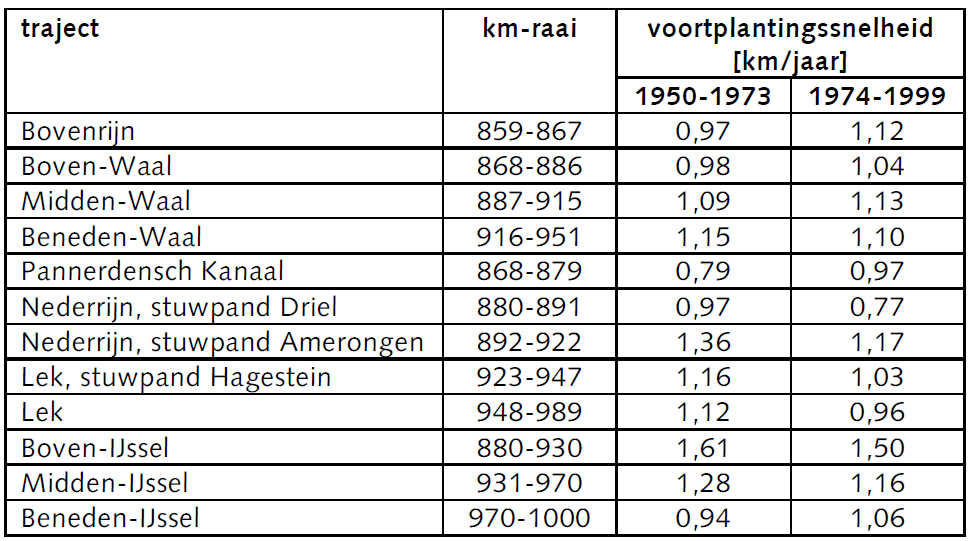
\includegraphics[width=\columnwidth]{figures/Tab2.png}
\caption{Overview of average bed celerities (based on km-averaged bed levels including the effects of dredging) by \citet{RIZA2005}.}
\label{Tab2Again}
\end{table}

\begin{table}
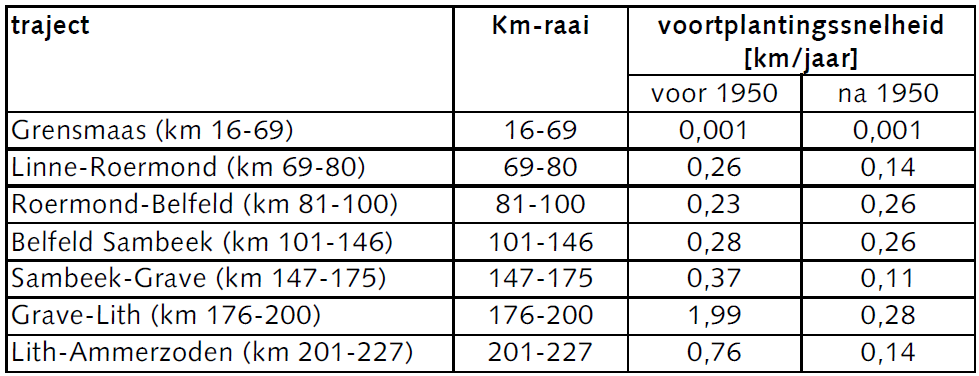
\includegraphics[width=\columnwidth]{figures/Tab3.png}
\caption{Overview of the reach averaged bed celerities (based on km-averaged bed levels including the effects of dredging) by \citet{Waterdienst2008}.}
\label{Tab3Again}
\end{table}

\begin{table}
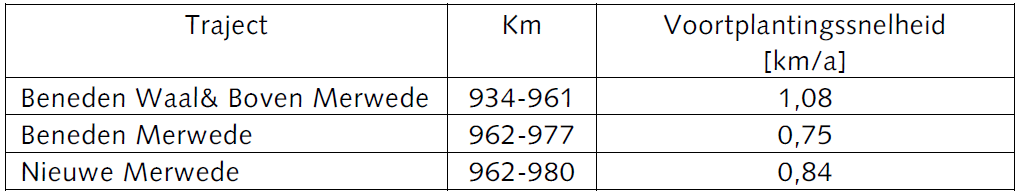
\includegraphics[width=\columnwidth]{figures/Tab4.png}
\caption{Overview of the reach averaged bed celerities (based on km-averaged bed levels for the period 1975-2000 including the effects of dredging) by \citet{RIZA2007}.}
\label{Tab4}
\end{table}

In order to translate these empirical year averaged values to discrete values per discharge block the following approximation is used for free flowing Rhine branches.
For the Bovenrijn discharges which are predominantly larger than 4000 m\textsuperscript{3}/s (during on average 8 \% of the year) a "high flow bed celerity" $w_h$ of 10 m/dag (3.65 km/yr) is used.

For discharge blocks which are predominantly below 4000 m\textsuperscript{3}/s a "low flow bed celerity" $w_l$ is used which is derived from the year-averaged bed celerity $\bar{c}$ as

\begin{equation}
w_l = \frac{\bar{c} - 0.082 \cdot 365}{0.918}
\label{Eq9}
\end{equation}

However, this approximation \autoref{Eq9} is only valid for the free flowing Rhine branches, hence it's for instance not valid for the Nederrijn where at low discharges the barriers are closed (\autoref{Fig6}).

\begin{figure}
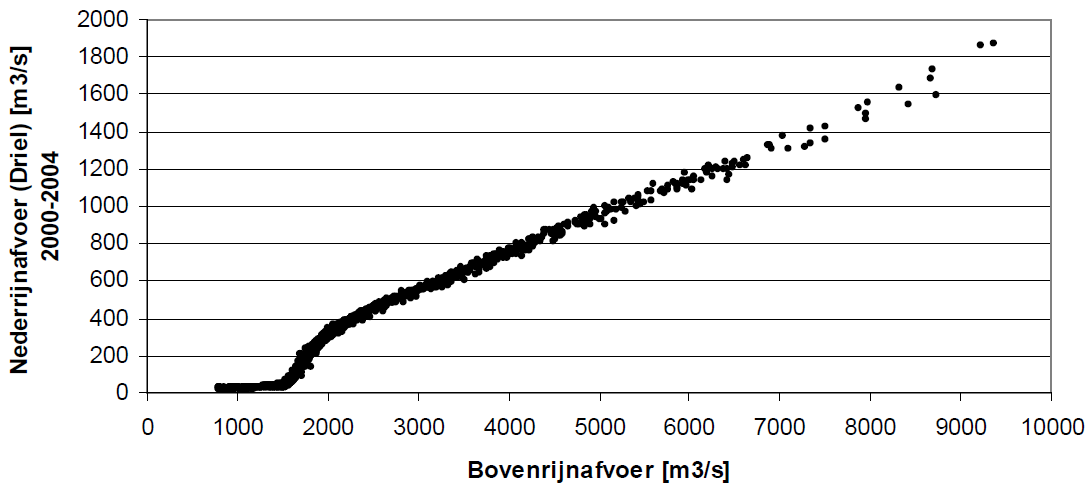
\includegraphics[width=\columnwidth]{figures/Fig6.png}
\caption{Nederrijn discharges at Driel-boven based on Donar database for the period 2000-2004).}
\label{Fig6}
\end{figure}

\autoref{Fig6} shows that the barriers in the Nederrijn are opened at a discharge of 1500 m\textsuperscript{3}/s in the Bovenrijn at Lobith (this value is exceeded during 57 \% of the year) and that the branch is approximately free flowing for discharges above 2200 m\textsuperscript{3}/s in the Bovenrijn at Lobith (exceeded during 33 \% of the year).
It's therefore assumed that the year-averaged bed celerity related to the low and high flow values as $\bar{c} = 0.082 w_h + (0.918 - 0.33) w_l$ such that for $w_h = 3,65$ km/yr we obtain

\begin{equation}
w_l = \frac{\bar{c} - 0.082 \cdot 3.65}{0.918 - 0.33}
\label{Eq10a}
\end{equation}

For the Meuse the we apply the following approximation.
It's assumed that the Meuse barriers are open for on average 10 days per year (3 \% of the time) such that the bed celerity can be estimated as

\begin{equation}
w_h = \frac{\bar{c}}{0,03}
\label{10b}
\end{equation}


Finally, due to the gradation the river bed of the Grensmaas will only become mobile at discharges above 1000 m\textsuperscript{3}/s which occurs on average about 4 days a year.
The bed celerity is thus estimated as

\begin{equation}
w_h = \frac{\bar{c}}{0,01}
\label{Eq10c}
\end{equation}

Based on the approximations \autoref{Eq9} to \autoref{Eq10c} and the year-averaged bed celerity values in \autoref{Tab2Again} to \autoref{Tab4} we obtain estimates for the bed celerities during high and low flow conditions.

\begin{table}
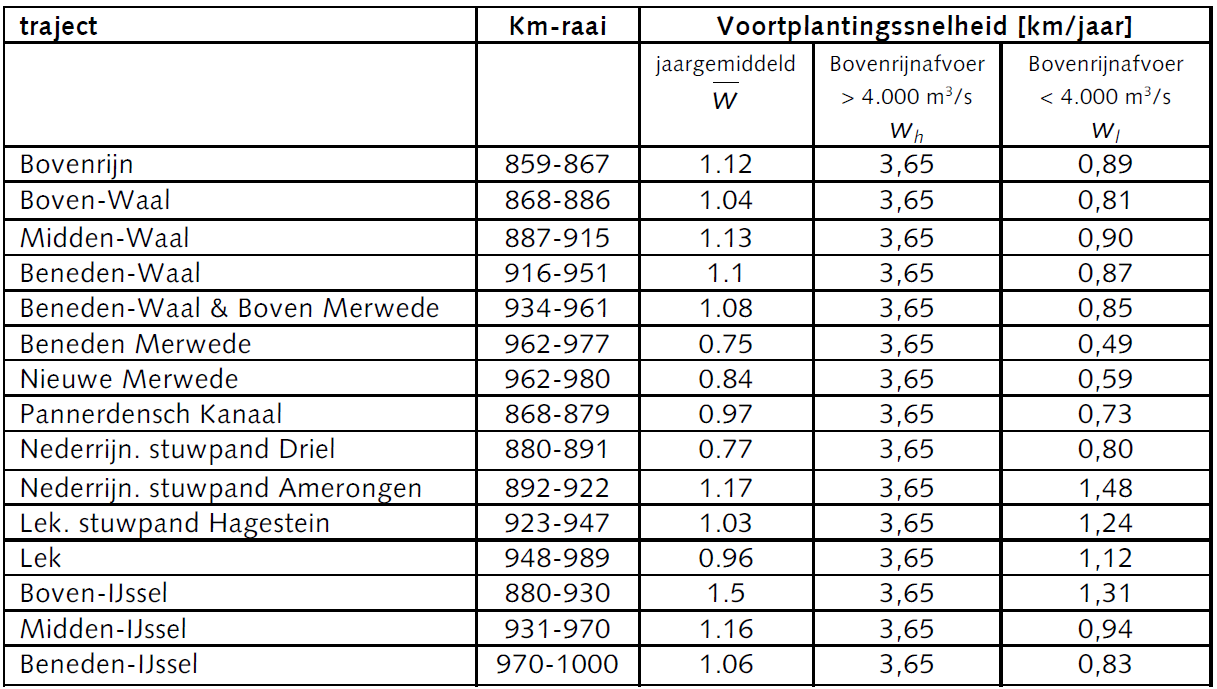
\includegraphics[width=\columnwidth]{figures/Tab4_the2nd.png}
\caption{Representative bed celerities during high- and low-flow conditions Rhine branches.}
\label{Tab4RT}
\end{table}

\begin{table}
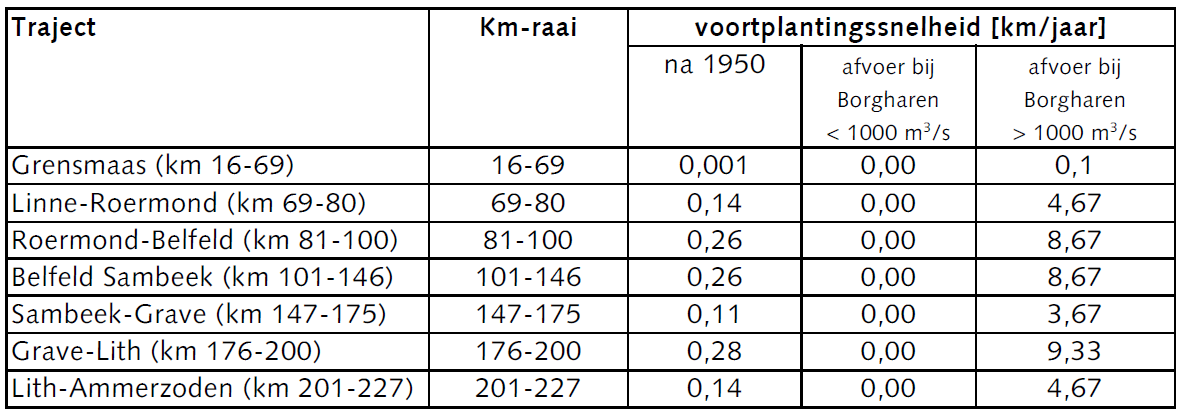
\includegraphics[width=\columnwidth]{figures/Tab5.png}
\caption{Representative bed celerities during high- and low-flow conditions Meuse.}
\label{Tab5}
\end{table}

\chapter{Steps in the analysis}\label{Chp:steps}

To apply \dfastmi one should carry out the following six steps.

\begin{enumerate}
\item Characterize the intervention to be evaluated using \dfmi.
Verify that it is appropriate to use \dfmi instrument; see \autoref{Chp:Guidance}.
Determine the branch and reach on which it is located; use the \dfmi GUI for this\footnote{The reaches are specified in the GUI both by a descriptive name and by an approximate indication of the river chainage.
Follow item \ref{reach_bnd} of \autoref{Sec:Limitations} if an intervention is located across or near a branch/reach boundary.}.
Determine the threshold discharge $Q_\text{thr}$ (at Lobith/Borgharen) at which the intervention (indirectly) starts to influence the flow pattern in the main channel.
The threshold discharge is critical for determining the fraction of the year that the intervention influences the flow, and hence the duration over which the bed level difference (compared to the reference situation) can develop.
As a result, this value is critical for determining the total volume of sedimentation (or erosion) that can be expected after one year.
Therefore, it is important to clearly specify how this threshold value has been determined.

\item Determine, given the branch/reach on which the intervention is location, which \dflowfm simulations should be carried out\footnote{Note that in WAQMORF and \dfmi version 2, the discharges depended on the characteristics of the intervention.
That is no longer the case.
The flow conditions are now fixed per river branch/reach.
Only the threshold discharge is relevant as this is the lowest discharge at which the intervention has any effect, and hence discharges below that value can be skipped.}.
The \dfmi GUI will provide you that list after selecting the appropriate branch/reach.
For the Dutch rivers these values are given by the following table
\newline
\newline
\begin{tabular}{l|l|l}
river & location & flow conditions \\ \hline
Rhine branches & Lobith & 1300, 2000, 3000, 4000, 6000, 8000 \SI{}{\metre\cubed\per\second}\\
Meuse & Borgharen & 750, 1300, 1700, 2100, 2500, 3200 \SI{}{\metre\cubed\per\second}
\end{tabular}
\newline
\newline
These flow conditions have been pre-configured for the latest \dflowfm schematizations.
It is not necessary to run simulations for conditions at which the intervention doesn't influence the flow patterns (i.e.~discharges associated with stagnant conditions due to closure of barriers, and discharges below the intervention specific $Q_\text{thr}$).
At this stage, \dfmi already reports the impacted length (`aanzandingslengte'), which is the distance over which a bed level change can built up during the period that the discharge of the river is above the threshold discharge.

\item Perform for each condition the hydrodynamic simulations for both the reference situation and the situation with intervention.
Verify that
\begin{itemize}
\item the \dflowfm results are stable
\item the intervention is properly represented on the mesh used (check a.o. proper alignment of groynes and levees, channel shape and bed roughness)
\item all simulations use the same base mesh (changes in dry areas may result in slight differences in the mesh effectively used)
\item there is a visible difference in the velocities in the main channel between the simulations with and without intervention
\end{itemize}

\item Run \dfastmi to compute for each grid point in the main channel, the following three variables

\begin{itemize}
\item year-averaged bed level change \unitbrackets{m} without dredging
\item maximum bed level change \unitbrackets{m} without dredging
\item minimum bed level change \unitbrackets{m} without dredging
\end{itemize}

once the (dynamic) equilibrium is reached. The year-averaged value is the main value for further analysis.
The minimum and maximum values indicate the variability of the bed level during an average year; this may provide critical insight for the stability of structures, such as groynes.
Note these values represent the morphological impact of the static intervention as defined in the \dflowfm schematisation when a (dynamic) equilibrium bed level is finally reached and maintenance dredging/dumping volumes are not adjusted to compensate.
Depending on the size of the impact and the morphological activity of the system, the new equilibrium may be reached quickly or very slowly over many years or decades.

\item The computational results are provided in \file{dfastmi\_results.nc} in the specified output folder and can be used to visualize the characteristic bed level changes in a graph and/or on a map.
Use patches with clearly defined colour scales for the overview.
Clip small bed level changes, e.g.~less than \SI{5}{\milli\metre}.
Create zoomed plots as appropriate with more detailed information, such as numeric values and isolines.
Add relevant information such as river chainage, navigation lane, and groynes/normal lines.

\item Estimate the yearly amount of dredging needed to counteract any sedimentation.
The first-year sedimentation volume is an estimate for the yearly amount of dredging needed to counteract any sedimentation as indicated in \autoref{Sec:DredgeVol}.
Since, if that volume is dredged after the first year, the river bed will be effectively reset to the initial condition, and the cycle will repeat.
For this estimate the user needs to accumulate the equilibrium bed level change (sedimentation) over the distance indicated by the impacted length starting from the upstream side of the impacted area.
If there are disjunct sedimentation areas, the accumulation should be carried out for each of the areas individually.
If areas are shorter than the impacted length, then the total equilibrium impact can be reached within one year.
\end{enumerate}

\chapter{Examples}

This chapter describes some examples of the \dfmi analysis.
The first two examples are taken from \citet{GiriJagers2022}.
That report tested a pilot implementation of \dfmi version 3 and used a number of slightly different hydrographs; the examples presented here use the final configuration as included in the \dfmi distribution.
The input files of the examples are included in the \file{examples} folder of the \dfmi distribution.

\section{Example 1: secondary channel along the Nederrijn}

For this first example, we compare the results of \dfastmi with the results of a morphological simulation using Delft3D-FLOW.
For consistency the \dfastmi analysis was performed using the hydrodynamic results of Delft3D-FLOW\footnote{Since \dfastmi expects \dflowfm results in netCDF UGRID format, the results were converted to the appropriate file format by means of \texttt{sim2ugrid}, see \autoref{Chp:Sim2Ugrid}.}.

For this analysis, the Nederrijn grid of the DVR model has been used.
The intervention concerns a secondary channel planned in the Palmerswaard which is located at Rkm 910-912 in the reach upstream of the Amerongen barrier at Rkm 922.
The reference model is based on the Baseline schematization ‘rijn-beno18\_5-v1’.
Since the DVR model was too coarse to represent the actual secondary channel, a combination of flow extraction (at Rkm 910.5) and insertion (at Rkm 912) was used to represent the side channel.

\begin{figure}
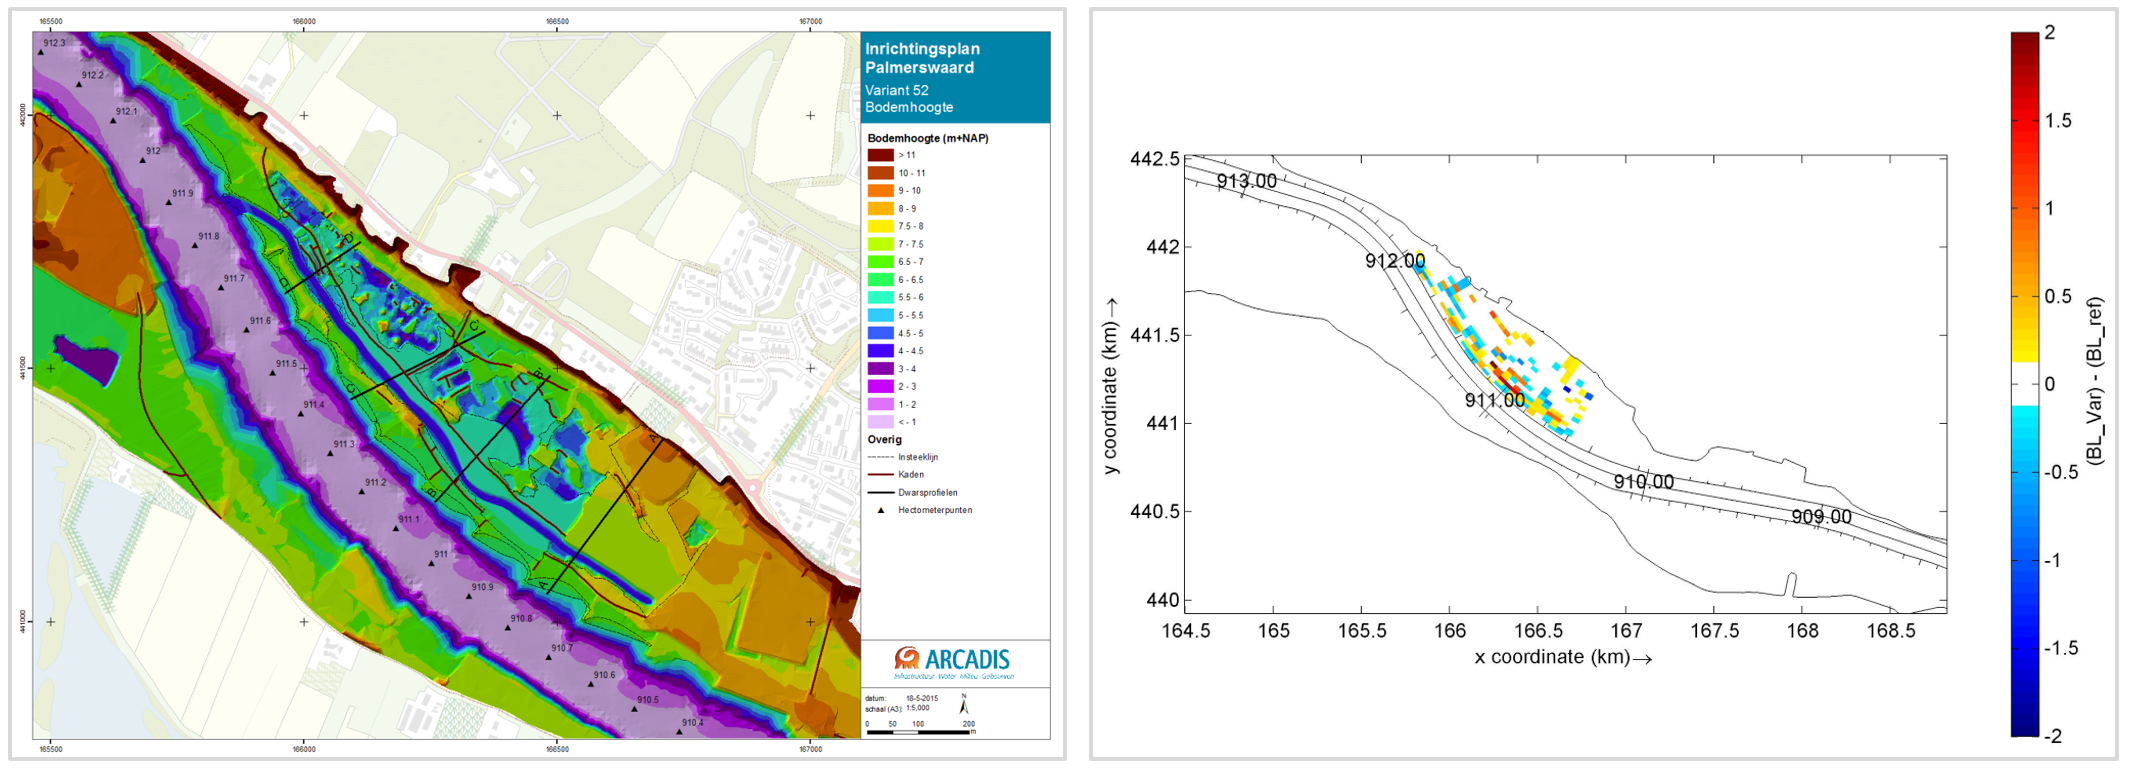
\includegraphics[width=\columnwidth]{figures/Palmerswaard_proj.png}
\caption{Side channel design (left) and initial representation on the grid (right).}
\label{Palmers_proj}
\end{figure}

Since the intervention is located on the Rhine branches, the new \dfastmi method requires the input of simulation results for 6 steady discharges: 1300, 2000, 3000, 4000, 6000, and \SI{8000}{\metre\cubed\per\second} at Lobith.
However, since the intervention is located in the backwater curve of the Amerongen barrier which is closed at discharges below \SI{1500}{\metre\cubed\per\second} causing largely stagnant flow conditions, the lowest discharge isn't relevant for this case.
Hence, \dfmi asks for the results of 10 simulations (5 discharges with and without intervention), see \autoref{Palmers_empty}.
After specifying all input files, the dialog will look like \autoref{Palmers_config} and if you save the configuration, the file will look as follows:

\begin{figure}
\center
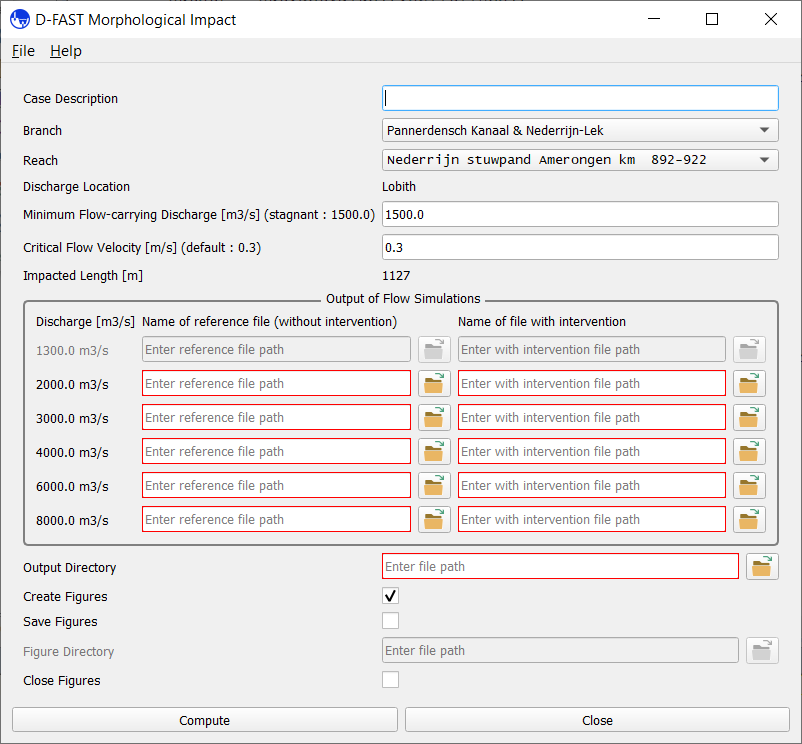
\includegraphics[width=11cm]{figures/Palmerswaard_empty.png}
\caption{Initial \dfmi screen after selecting the appropriate branch and reach.}
\label{Palmers_empty}
\end{figure}

\begin{figure}
\center
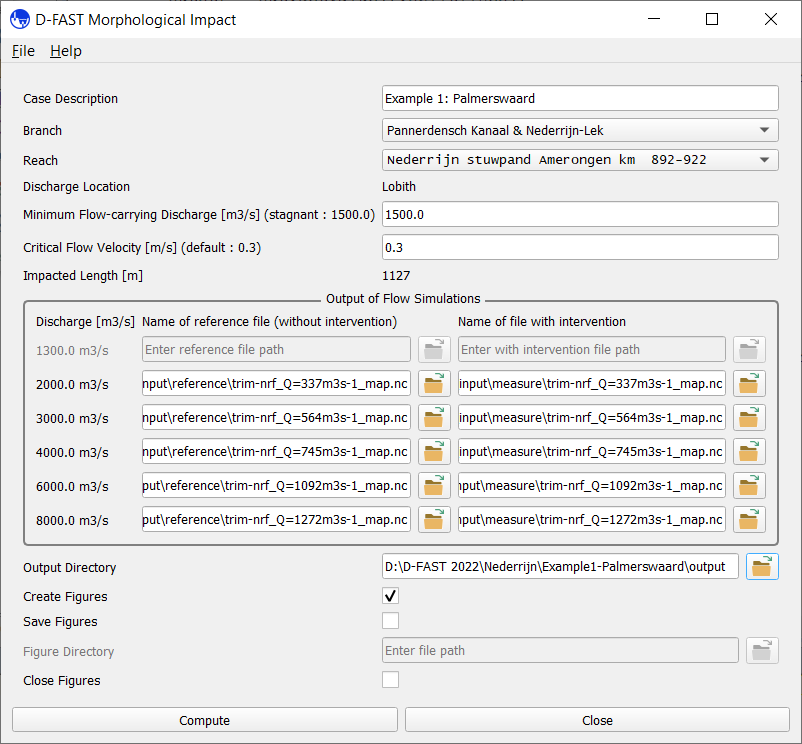
\includegraphics[width=11cm]{figures/Palmerswaard_config.png}
\caption{\dfmi screen after specifying all files.}
\label{Palmers_config}
\end{figure}

\verbfilenobox[\scriptsize]{../examples/01 - Palmerswaard/example1.cfg}

The \dfmi analysis is performed when you click on the \button{Compute} button.
The program will show a message that the analysis has successfully ended, and that a report.txt file has been written to the output folder.
Furthermore, since we have selected the "Create Figures" option, it will create a rudimentary overview picture of the change in the year-averaged equilibrium bed level that the result of the intervention.
The initial view will cover the whole model area as shown in \autoref{Palmers_fig}.
You can zoom in on the area of interest as shown in \autoref{Palmers_fig_zoomed}.
See \autoref{Sec:FigNavigation} for navigating these figures.
The content of the report file is shown below:

\begin{figure}
\center
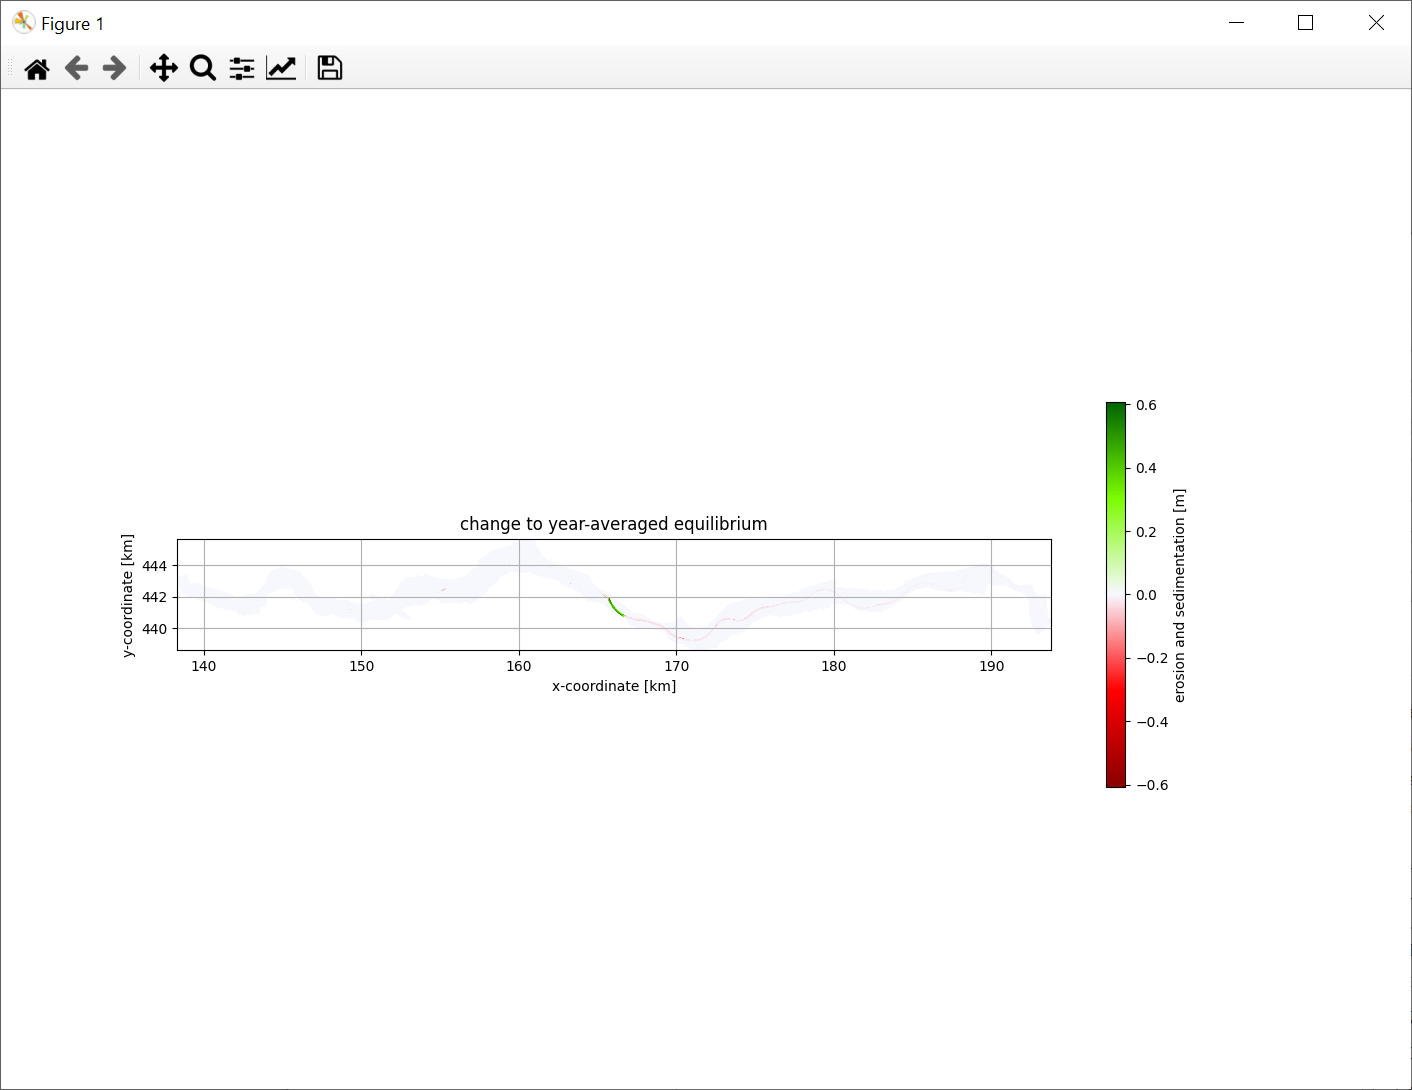
\includegraphics[width=\textwidth]{figures/Palmerswaard_fig.png}
\caption{Initial view of the analysis results.}
\label{Palmers_fig}
\end{figure}

\begin{figure}
\center
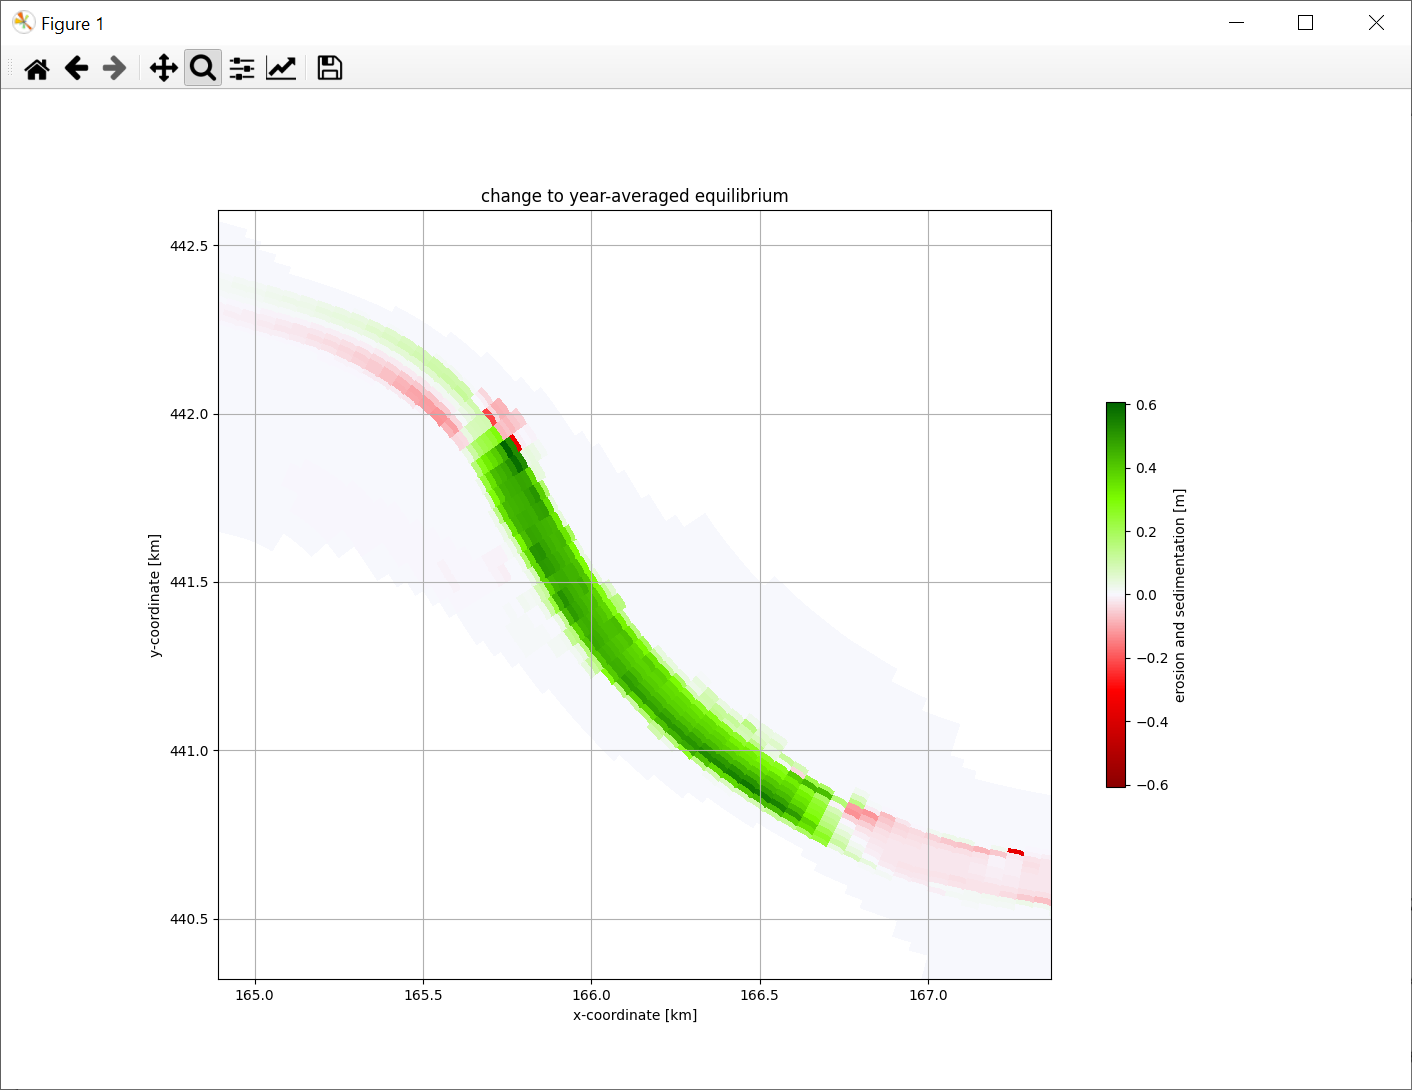
\includegraphics[width=\textwidth]{figures/Palmerswaard_fig_zoomed.png}
\caption{Zoomed view of the analysis results.}
\label{Palmers_fig_zoomed}
\end{figure}

\verbfilenobox[\scriptsize]{../examples_references/01 - Palmerswaard/output/report.txt}

\autoref{Palmers_mor} shows the results of a reference morphology simulation using Delft3D 4 (for details, see \citet{GiriJagers2022}).
The figure shows the morphological evolution of the Delft3D simulation.
The overall \dfastmi results compare well with the long term (12yr) Delft3D simulation although the asymmetry downstream of the main sedimentation patch differs.

\begin{figure}[H]
\center
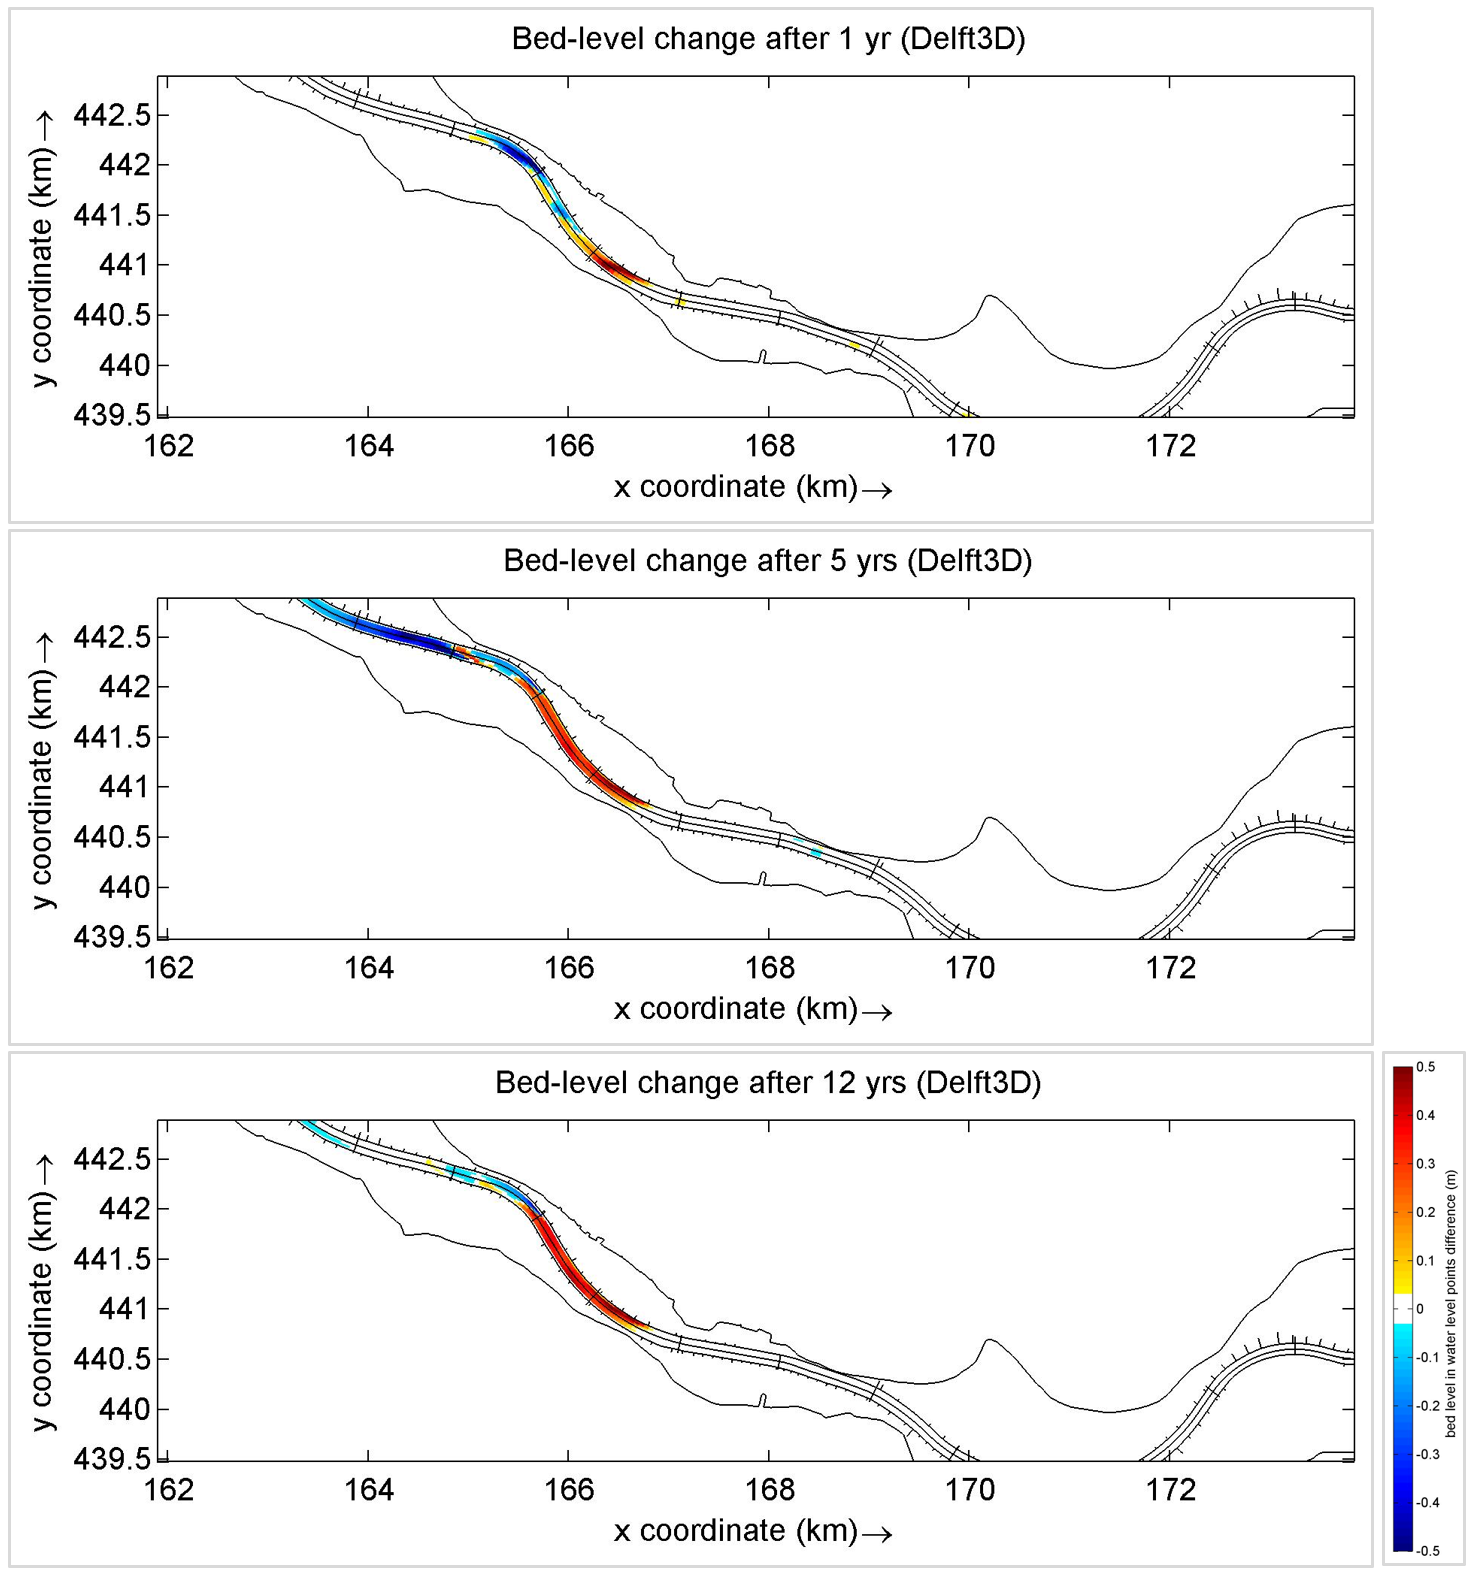
\includegraphics[width=\textwidth]{figures/Palmers_mor.png}
\caption{The bed-level difference between the variant and the reference after 1, 5 and 12 years of morphological simulation.}
\label{Palmers_mor}
\end{figure}


\section{Example 2: secondary channel along the Pannerdensch Kanaal}

For this second example, we follow the same approach as example 1: we compare the results of \dfastmi with the results of a morphological simulation using Delft3D-FLOW.
The model was based on the DVR model, but the domain was reduced to focus mainly on the Pannerdensch Kanaal \citep{BomLeeuwen2020}.
Because of the two bifurcations upstream and downstream, it still included parts of all the branches (Bovenrijn, Pannerdensch Kanaal, Waal, Nederrijn and IJssel).
Only results for the Pannerdensch Kanaal will be presented here.

The intervention concerns a secondary channel `green river' implemented along the right bank at Rkm 871-872 just downstream of Pannerden.
The reference model is based on the Baseline schematization ‘rijn-beno18\_5-v1’.
Again, a combination of flow extraction and insertion was used to represent the side channel because the secondary channel wasn't represented accurately on the grid.

\begin{figure}
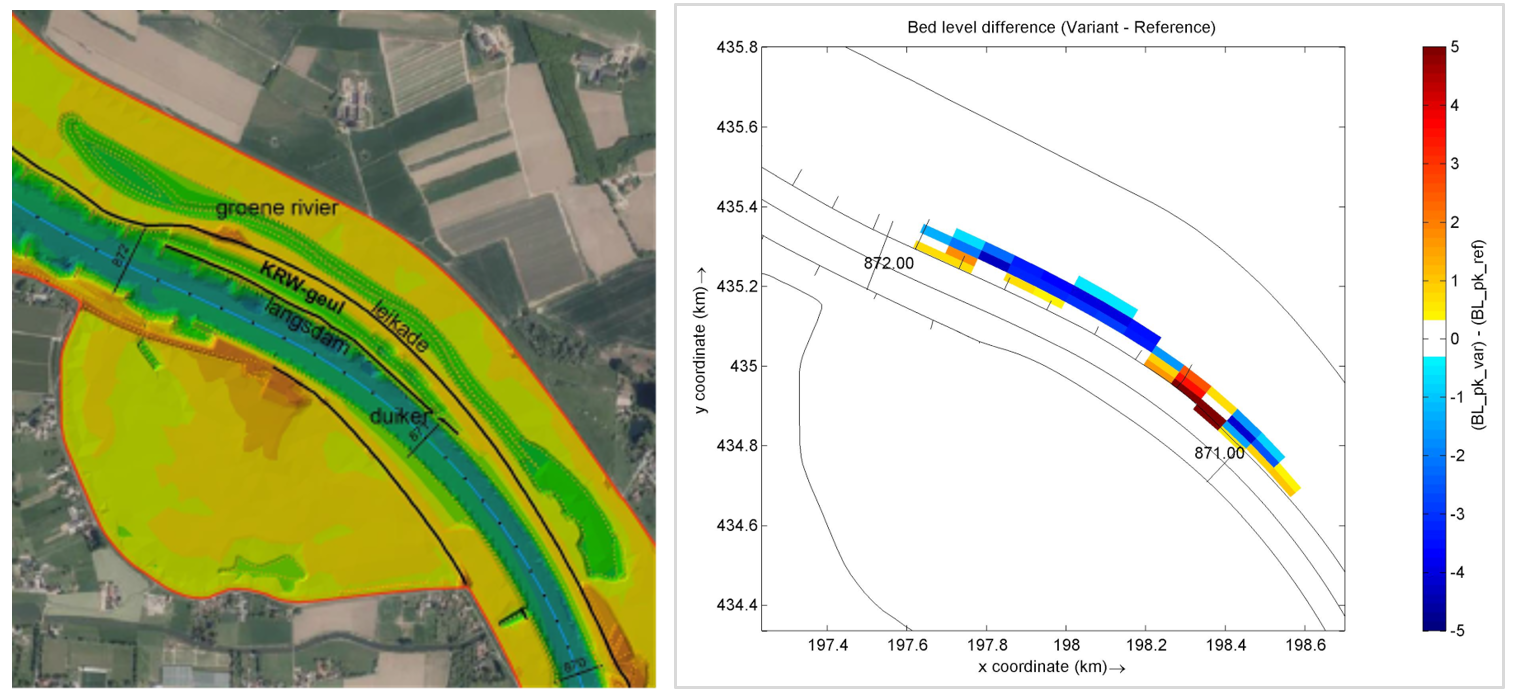
\includegraphics[width=\columnwidth]{figures/Pannerden_proj.png}
\caption{Side channel design (left) and initial representation on the grid (right).}
\label{Pannerden_proj}
\end{figure}

Since the intervention is located on the Rhine branches, the new \dfastmi method requires the input of simulation results for 6 steady discharges: 1300, 2000, 3000, 4000, 6000, and \SI{8000}{\metre\cubed\per\second} at Lobith.
Contrary to example 1, the lowest discharge is relevant for this case.
Hence, \dfmi asks for the results of 12 simulations (6 discharges with and without intervention).
After specifying all input files, the dialog will look like \autoref{Pannerden_config} and if you save the configuration, the file will look as follows:

\begin{figure}
\center
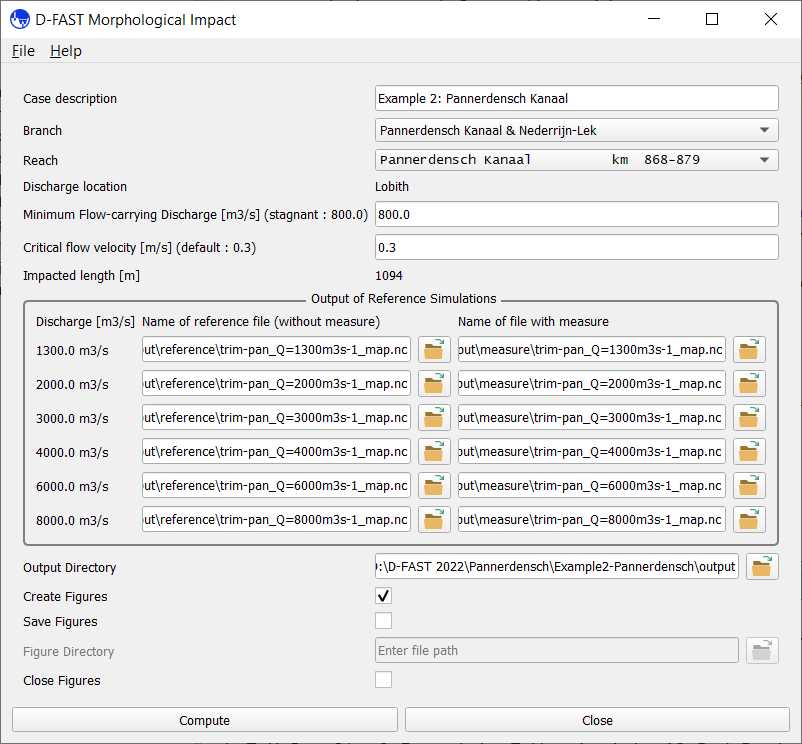
\includegraphics[width=11cm]{figures/Pannerden_config.png}
\caption{\dfmi screen after specifying all files.}
\label{Pannerden_config}
\end{figure}

\verbfilenobox[\scriptsize]{../examples/02 - Pannerdensch Kanaal/example2.cfg}

The \dfmi analysis is performed when you click on the \button{Compute} button.
The program will show a message that the analysis has successfully ended, and that a report.txt file has been written to the output folder.
Furthermore, since we have selected the "Create Figures" option, it will create a rudimentary overview picture of the change in the year-averaged equilibrium bed level that the result of the intervention.
A zoomed-in version of that figure is shown in \autoref{Pannerden_fig_zoomed}.
See \autoref{Sec:FigNavigation} for navigating these figures.
The content of the report file is shown below:

\begin{figure}
\center
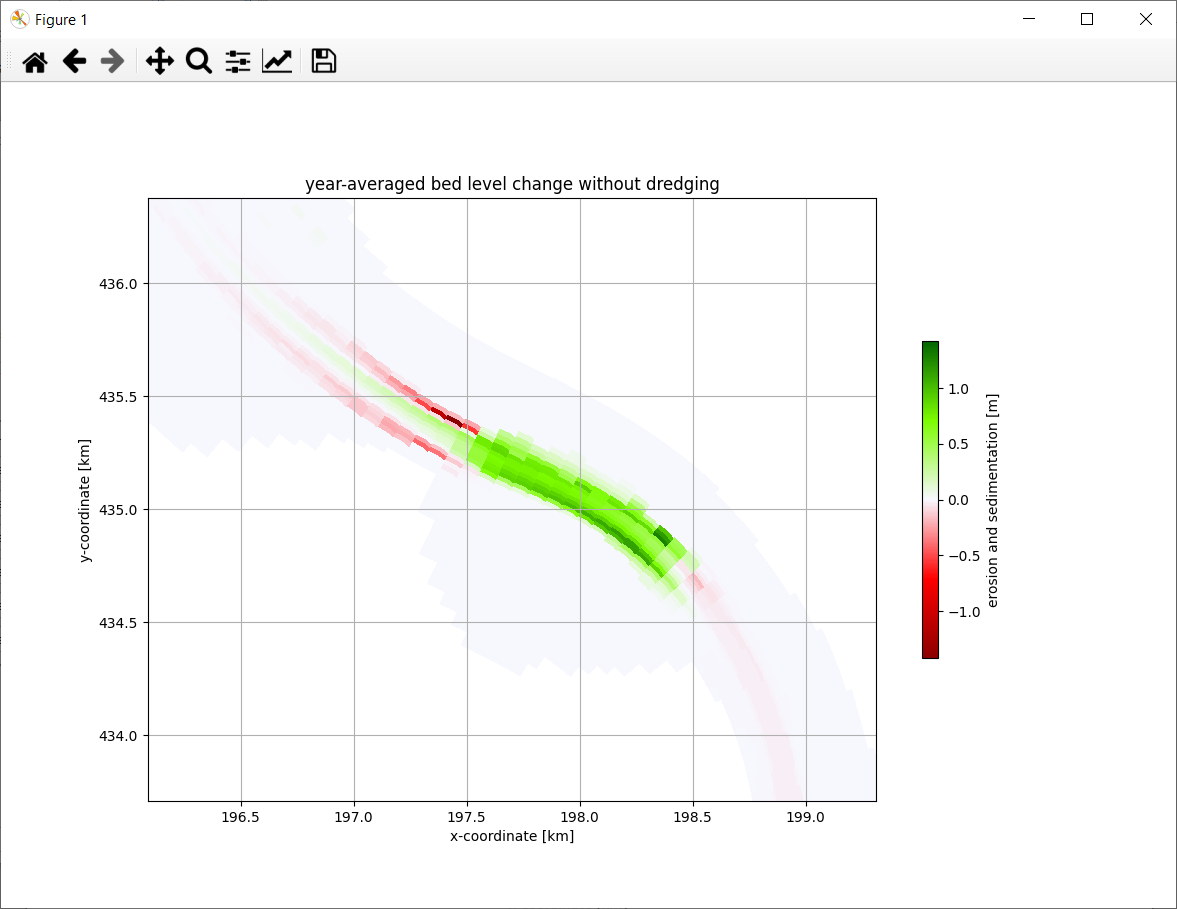
\includegraphics[width=\textwidth]{figures/Pannerden_fig_zoomed.png}
\caption{Zoomed view of the analysis results.}
\label{Pannerden_fig_zoomed}
\end{figure}

\verbfilenobox[\scriptsize]{../examples_references/02 - Pannerdensch Kanaal/output/report.txt}

\autoref{Pannerden_mor} shows the results of a reference morphology simulation using Delft3D 4 (for details, see \citet{GiriJagers2022}).
The figure shows the morphological evolution of the Delft3D simulation.
The overall \dfastmi results compare well with the long term (15yr) Delft3D simulation although \dfmi suggests sedimentation in the centre of the channel downstream of the main sedimentation area whereas the morphological simulation doesn't show that behaviour.

\begin{figure}[H]
\center
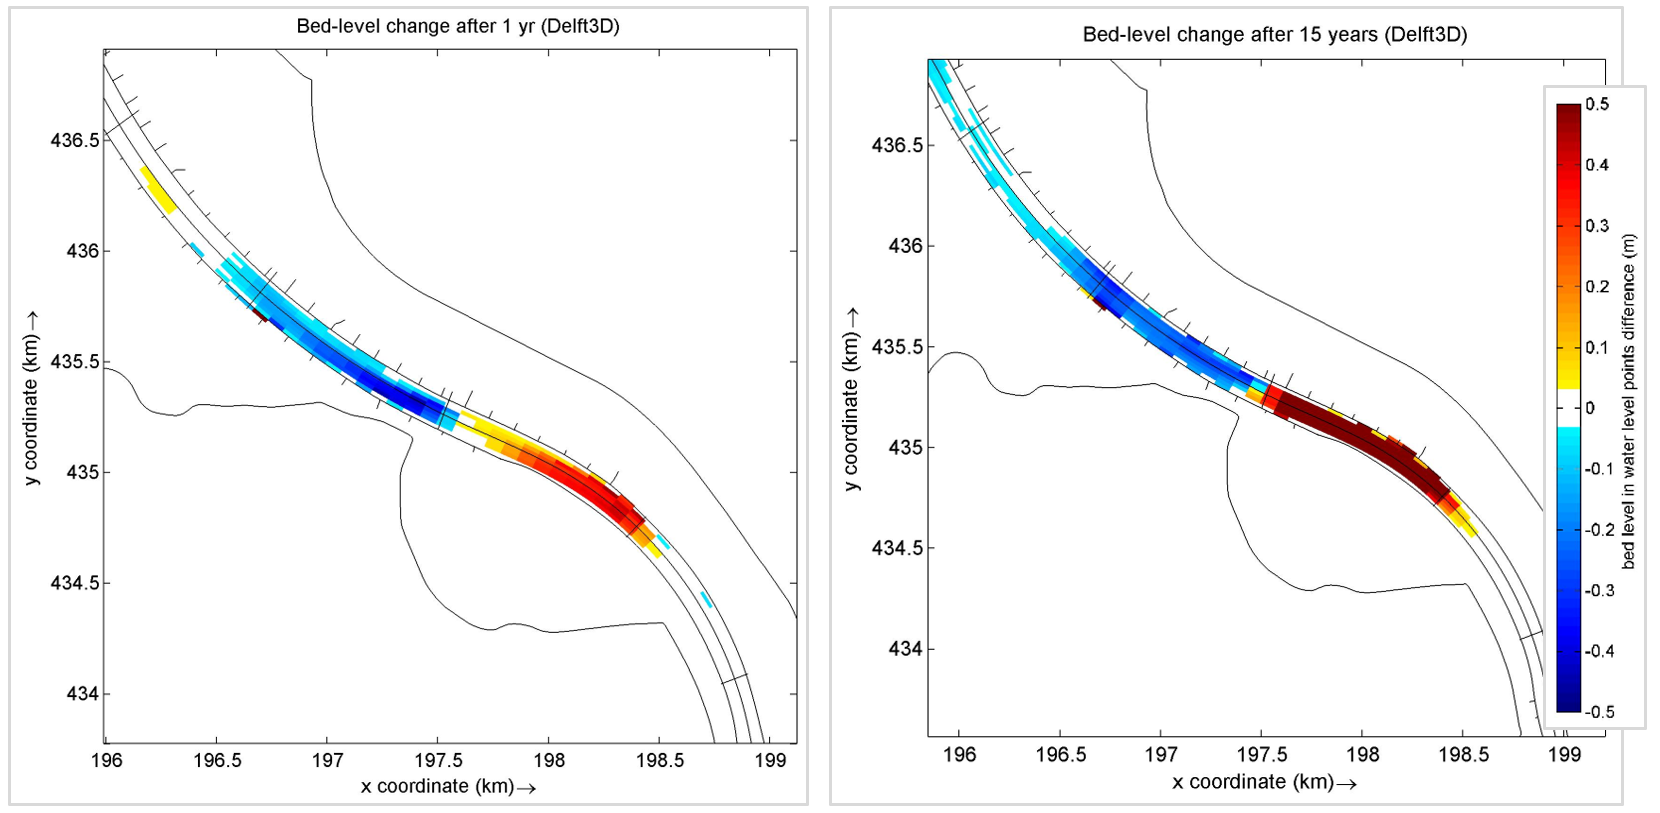
\includegraphics[width=\textwidth]{figures/Pannerden_mor.png}
\caption{The bed-level difference between the variant and the reference after 1 and 15 years of morphological simulation.}
\label{Pannerden_mor}
\end{figure}

%\textit{}\include{chapters_usermanual/guide}

\nonumchapter{References}
\bibliography{dfastmi}

\appendix
\chapter{File formats}

The software distinguishes 6 files:

\begin{itemize}
\item The \emph{rivers configuration file} defines the branches and reaches, and all parameter settings specific for the overall system, per branch or per reach.
\item The \emph{dialog text file} defines all strings to be used in the interaction with the users (GUI, report, or error messages).
\item The \emph{analysis configuration file} defines the settings that are relevant for a specific execution of the algorithm, i.e.~for a specific branch, reach and intervention.
\item The \emph{simulation result files} define the spatial variations in the velocities and water depths as needed by the algorithm.
\item The \emph{report file} contains a logging of the settings and lumped results for the analysis.
\item The \emph{spatial output file} contains the estimate of the spatial variation in the sedimentation and erosion patterns that will result from the intervention (minimum, mean and maximum).
\end{itemize}

Each file type is addressed separately in the following subsections.

\section{Rivers configuration file}

The rivers configuration file follows the common ini-file format.
The file must contain a \keyw{[General]} block with a keyword \keyw{Version} to indicate the version number of the file.
The version number should be \keyw{3.0}.\footnote{Initially this file version was named \keyw{2.0} but to avoid confusion with the fact that this file format is only supported by \dfastmi version 3.0, the version number has been increased.
Files with version \keyw{2.0} are still accepted, but not recommended.}

Besides the \keyw{[General]} block version 3.0 files should only contain data blocks identifying the river branches (in Dutch: takken).
The names of those blocks will be used as branch names.
For instance, a block [My branch] will be processed as a branch called "My branch".
The order of the branches in the gui will correspond to the order of the blocks in the file.
The branch block defines the reaches (in Dutch: stukken) to be distinguished as well as the branch or reach specific parameter settings.
The \keyw{[General]} block may contain default values for the various parameters.
Further details follow below.

\begin{longtable}{l|l|p{8cm}}
\caption{Description of rivers configuration version 3} \\
Block & Keyword & Description \\ \hline
\endfirsthead
\multicolumn{3}{l}{\textsl{(continued from previous page)}} \\
Block & Keyword & Description \\ \hline
\endhead
\hline \multicolumn{3}{r}{\textsl{(continued on next page)}} \\
\endfoot
\endlastfoot
\keyw{General} & \keyw{Version} & Version number.
Should be \keyw{3.0}. \\
\keyw{General} & \keyw{checksum} & Checksum of the rivers configuration file.
Used to verify that the rivers configuration file wasn't accidentally modified. \\
BranchName<i> & \keyw{QLocation} & Location at which discharges for branch <i> are defined. \\
BranchName<i> & \keyw{Reach<j>} & Name of reach <j> within branch <i>. \\
\keyw{*} & \keyw{NWidth} & Normal width \unitbrackets{m} of main channel. \\
\keyw{*} & \keyw{QStagnant} & Discharge \unitbrackets{m\textsuperscript{3}/s} below which main channel flow can be assumed stagnant. \\
\keyw{*} & \keyw{UCrit} & Critical (minimum) velocity \unitbrackets{m/s} for sediment transport. \\

\keyw{*} & \keyw{HydroQ} & Series of discharges \unitbrackets{\SI{}{\metre\cubed\per\second}} representing each stage of the ``hydrograph''. \\
\keyw{*} & \keyw{Tide} & Flag to indicate whether the stages of the ``hydrograph'' are represented by discharge only (False) or by a combination of discharge and tide (True). \\
\keyw{*} & \keyw{TideBC} & Series of other tidal conditions representing the stages of the ``hydrograph''.
Only used in case \keyw{Tide} equals True. \\

\keyw{*} & \keyw{AutoTime} & Flag to indicate whether the duration of each discharge period should automatically be derived from the exceedance curve given by \keyw{QFit}.
The default value is False. \\
\keyw{*} & \keyw{HydroT} & Series of values specifying the duration of each stage of the ``hydrograph''.
The unit used for specifying the durations is arbitrary: the sum of all durations is assumed to be equivalent to 1 year.
The length of the series should be equal to the length of the series of discharges specified for \keyw{HydroQ}.
Only used in case \keyw{AutoTime} equals False. \\
\keyw{*} & \keyw{QFit} & Two discharges \unitbrackets{\SI{}{\metre\cubed\per\second}} used for representing the exceedance curve in case \keyw{AutoTime} equals True. \\

\keyw{*} & \keyw{CelerForm} & Flag to indicate the method used for determining the bed celerity.
The options are 1 (series of discharge, bed celerity pairs) and 2 (power-law relation between celerity and discharge).
The default value is 2. \\
\keyw{*} & \keyw{PropQ} & Strictly-monotonous increasing list of discharges \unitbrackets{\SI{}{\metre\cubed\per\second}} for which the bed celerity is given.
Only used in case \keyw{CelerForm} equals 1. \\
\keyw{*} & \keyw{PropC} & List of bed celerities \unitbrackets{\SI{}{\metre\per\second}} one value for each discharge specified by \keyw{PropQ}.
The length of the lists given by \keyw{PropQ} and \keyw{PropC} should be equal.
Only used in case \keyw{CelerForm} equals 1. \\
\keyw{*} & \keyw{CelerQ} & Two values representing the multiplication scalar and exponent of the power-law relation of the bed celerity \unitbrackets{\SI{}{\metre\per\second}} as function of the discharge \unitbrackets{\SI{}{\metre\cubed\per\second}}.
Only used in case \keyw{CelerForm} equals 2.
\end{longtable}

All keywords listed for block \keyw{*} may occur either in the \keyw{[General]} block or in one of the branch specific blocks where they may optionally be concatenated with the reach number <j>.
Those keywords may thus occur in three flavours:

\begin{enumerate}
\item Plain keyword in block \keyw{[General]}: global default value valid for all branches
\item Plain keyword in branch specific block: default value for that branch (overrules any global default)
\item Keyword followed by reach number <j> in branch specific block: value valid for that specific reach (on that branch).
\end{enumerate}

\subsubsection*{Example}

The following excerpt of the default \keyw{Dutch\_rivers.ini} configuration file shows the \keyw{[General]} as well as the first part of the \keyw{[Bovenrijn \& Waal]} block for the first branch.
It includes a global value of 0.3 for \keyw{UCrit} and 100 for \keyw{QMin}.
The other parameters are specified at branch level and mostly uniform for the whole branch.
Only \keyw{NWidth} and \keyw{PRLow} vary depending on the reach selected.

\begin{Verbatim}
    [General]
        Version    = 3.0
        UCrit      = 0.3
        CelerForm  = 1
        checksum   = 2377805458
    
    [Bovenrijn & Waal]
        QLocation  = Lobith
        HydroQ     = 1300 2000 3000 4000 6000 8000
        AutoTime   = True
        QStagnant  = 800
        QFit       = 800  1280
    
        Reach1     = Bovenrijn                    km  859-867
        NWidth1    = 340
        PropQ1     = 3500  3501
        PropC1     = 0.89  3.65
    
        Reach2     = Boven-Waal                   km  868-886
        NWidth2    = 260
        PropQ2     = 3500  3501
        PropC2     = 0.81  3.65

        ... continued ...
\end{Verbatim}

\section{Dialog text file}

The dialog text file uses the block labels enclosed by square brackets of the common ini-file format, but the lines in between the blocks are treated verbatim and don't list keyword/value pairs.
Every print statement in the program is associated with a short descriptive identifier.
These identifiers show up in the dialog text file as the block labels.
The text that follows the block label will be used at that location in the program.
The order of the blocks in the file is not important.
Please note that every line is used as is, so don't add indentations or blank lines unless you want those to show up during the program execution.
Most blocks may contain any number of lines, but some blocks may only contain a single line in particular block that start with \keyw{gui\_} or \keyw{filename\_}.
Some data blocks may contain one or more named placeholders, e.g. \keyw{{version}}, used for inserting values by means of the Python \keyw{format()} method.

\subsubsection*{Example}

The following excerpt of the default \keyw{messages.NL.cfg} dialog text file shows the string definition for 5 identifiers, namely '' (the identifier for an empty line), 'header', 'confirm', 'confirm\_or' and 'confirm\_or\_restart'.
The header string contains one placeholder, namely \keyw{{version}} for the the version number.

\begin{Verbatim}
    []
    
    [reduce_output]
    The option 'reduce_output' is active.
    
    [header]
    D-FAST Morphological Impact implements an algorithm to estimate the local
    morphological effects of a local intervention (i.e. an adjustment to the
    river). The conceptual framework was originally introduced in
        "RWS-WD memo WAQUA vuistregel 20-10-08"
    but it has been extended and improved over the years. Check the user manual
    for the details of the currently implemented algorithm.
    
    It is based on an estimation of the equilibrium bed level changes in the main
    channel that would occur eventually when river maintenance would not be
    adjusted.
    
    The effect is expressed as:
    
        year-averaged bed level change [m] without dredging
        maximum bed level change [m] without dredging
        minimum bed level change [m] without dredging
    
    By means of these estimates bottlenecks can be identified. The results are not
    suitable for direct estimation of the impact on the maintenance of the
    navigation channel!
    
    The combination of the total equilibrium sedimentation volume and the yearly
    sediment load of the river determines the period over which the equilibrium
    can be reached.
    
    
    This is version {version}.
    
    [confirm]
    Confirm using "y" ...
    
    [confirm_or]
    Confirm using "y", or reply "n" ...
    
    ... continued ...
\end{Verbatim}

\section{Analysis configuration file}\label{app:config}

The analysis configuration file follows the common ini-file format.
The file must contain a \keyw{[General]} block with a keyword \keyw{Version} to indicate the version number of the file.
The version number should be \keyw{3.0}.\footnote{Initially this file version was named \keyw{2.0} but to avoid confusion with the fact that this file format is only supported by \dfastmi version 3.0, the version number has been increased.
Files with version \keyw{2.0} are still accepted, but not recommended.}

Version 3.0 files must contain in the \keyw{[General]} block also the keywords \keyw{Branch} and \keyw{Reach} to identify the branch (in Dutch: tak) and reach (in Dutch: stuk) in which the intervention is located.
The specified names may be shortened, but they should uniquely identify the branch and reach amongst the names of the other branches and reaches.
The same block may also contain \keyw{QThreshold} and \keyw{UCrit} values representative for this particular intervention if they differ from those typical for the selected reach.
Furthermore, this block may contain \keyw{FigureDir} and \keyw{OutputDir} specifying where the figures and other output files should be written.
The \keyw{RiverKM} keyword to specify the chainage along the reach of interest is needed for estimating the initial year dredging volumes.
Last but not least, the user needs to specify the names of the D-Flow FM map- or fourier-files containing the results of the simulations without intervention (reference) and with intervention for the selected flow conditions.
These names must be specified in a continuous sequences of numbered blocks named \keyw{C1}, \keyw{C2}, etc.
The order of the blocks is not important: the relevant blocks are identified by means of the \keyw{Discharge} and optionally \keyw{TideBC} specified per block.
There should be a match for every stage of the configured ``hydrograph'' for the selected branch/reach.
The file names may be specified using relative or absolute paths.

\begin{tabular}{l|l|p{8cm}}
Block & Keyword & Description \\ \hline
\keyw{General} & \keyw{Version} & Version number.
Should be \keyw{3.0}. \\
\keyw{General} & \keyw{CaseDescription} & Description of the analysis. \\
\keyw{General} & \keyw{Branch} & Name of the selected branch. \\
\keyw{General} & \keyw{Reach} & Name of the selected reach. \\
\keyw{General} & \keyw{QThreshold} & Minimum discharge \unitbrackets{\SI{}{\metre\cubed\per\second}} at which intervention becomes active. \\
\keyw{General} & \keyw{UCrit} & Critical (minimum) velocity \unitbrackets{\SI{}{\metre\per\second}} for sediment transport. \\
\keyw{General} & \keyw{RiverKM} & Name of file with river chainage \unitbrackets{\SI{}{\kilo\metre}} and corresponding xy-coordinates. \\
\keyw{General} & \keyw{FigureDir} & Directory for storing figures (default relative to work dir: figure). \\
\keyw{General} & \keyw{OutputDir} & Directory for storing output files. \\
\keyw{C}<i> & \keyw{Discharge} & Discharge \unitbrackets{m\textsuperscript{3}/s} of condition <i>. \\
\keyw{C}<i> & \keyw{TideBC} & Tidal boundary of condition <i>. \\
\keyw{C}<i> & \keyw{Reference} & Name of D-Flow FM map- or fourier-file to be used for reference condition <i>. \\
\keyw{C}<i> & \keyw{WithIntervention} & Name of D-Flow FM map- or fourier-file that includes the intervention <i>. \\
\end{tabular}

\subsubsection*{Example}

This example shows a complete analysis configuration file for an intervention in the first branch/reach of the default \keyw{Dutch\_rivers.cfg} configuration.
It reports the default settings.
Only the \keyw{Version}, \keyw{Branch}, \keyw{Reach}, \keyw{Reference} and \keyw{WithIntervention} keywords are required for the full analysis.

\begin{Verbatim}
    [General]
      Version          = 3.0
      CaseDescription  = 
      Branch           = Bovenrijn & Waal
      Reach            = Boven-Waal                   km  868-886
      Qthreshold       = 1000.0
      Ucrit            = 0.3
      OutputDir        = 
      Plotting         = False
      SavePlots        = False
      FigureDir        = 
      ClosePlots       = False
      RiverKM          = 
    
    [C1]
      Discharge        = 1300.0
      Reference        = Case42/Q1/Reference/DFM_OUTPUT_Q1/Q1_map.nc
      WithIntervention = Case42/Q1/Updated/DFM_OUTPUT_Q1/Q1_map.nc
    
    [C2]
      Discharge        = 2000.0
      Reference        = Case42/Q2/Reference/DFM_OUTPUT_Q2/Q2_map.nc
      WithIntervention = Case42/Q2/Updated/DFM_OUTPUT_Q2/Q2_map.nc
    
    [C3]
      Discharge        = 3000.0
      Reference        = Case42/Q3/Reference/DFM_OUTPUT_Q3/Q3_map.nc
      WithIntervention = Case42/Q3/Updated/DFM_OUTPUT_Q3/Q3_map.nc

        ... continued ...
\end{Verbatim}

\section{Simulation result files}

\dfastmi expects all data in UGRID netCDF file similar to the map-file output of \dflowfm.
\dfastmi reads the results directly no conversion is necessary.
These files may contain multiple time steps; the final time steps will be used for the analysis.
The mesh geometry is transferred from one of the simulation files to the \dfastmi spatial output "results" file.

\section{Report file}

\dfastmi will write a report of the analysis.
This report file is a simple text file consistent with the earlier reports written by WAQMORF.
The length and content of the report vary depending on the availability of the simulation result files and the language selected.


\section{Spatial output file}

\dfastmi generates one UGRID netCDF file containing the spatial results of the analysis.
The mesh information is copied from the first D-Flow FM map- or fourier-file read, and the three data fields (erosion and sedimentation patterns for mean, minimum, and maximum impact) follow standardized conventions for data stored at cell centres (\keyw{face}-values) on an unstructured mesh.
As a result the data may be visualized using a number of visualization tools such as QUICKPLOT and QGIS.

\chapter{Interoperability} \label{Chp:Sim2Ugrid}

\dfastmi reads data from 2D UGRID/CF netCDF files such as written by \dflowfm.
Other software may also write their netCDF result following the general \href{https://cfconventions.org/}{CF (Climate \& Forecasting)} and \href{http://ugrid-conventions.github.io/ugrid-conventions/}{UGRID} conventions.
In the following sections we discuss to which degree \dfmi depends on \dflowfm specific choices, and how to convert the output of other models to the format supported by \dfmi.

\section{File format assumptions}

Simulation files (both with and without measure) should contain \emph{one} 2D UGRID mesh variable.
These variables must be identifiable by means of the attributes \keyw{cf\_role = mesh\_topology} and \keyw{topology\_dimension = 2}.
The \keyw{face\_node\_connectivity} attribute of this variable must point to the face-node connectivity of the 2D mesh.
The \keyw{node\_coordinates} attribute must point to the x,y coordinates of the nodes; currently.
For geospatial operations (research functionality) \dfmi assumes that the coordinates are projected coordinates in metres.

The file must contain one or more time steps for the following quantities:
\begin{itemize}
\item depth-averaged flow velocity vector defined on the faces of the mesh, identifiable by means of the CF standard names \keyw{sea\_water\_x\_velocity} and \keyw{sea\_water\_y\_velocity}, and attributes \keyw{mesh} pointing to the mesh variable and \keyw{location = face}.
\item water depth defined on the faces of the mesh, identifiable by means of the CF standard name \keyw{sea\_floor\_depth\_below\_sea\_surface}, and attributes \keyw{mesh} pointing to the mesh variable and \keyw{location = face}.
\end{itemize}

\section{File conversion}

The formal working order is to base the \dfastmi analysis on the results of \dflowfm simulations.
However, sometimes it may be useful to use results obtained from other hydrodynamic models, such as Delft3D-FLOW or WAQUA (SIMONA).
This pathway has in particular been used to validate the \dfmi analysis using Delft3D flow results against Delft3D morphological simulations using the same model configuration.
For this purpose, a tool \keyw{sim2ugrid} has been made that converts Delft3D-FLOW (trim-files) or WAQUA results (SDS-files) to 2D UGRID/CF netCDF files accepted by \dfmi.
This tool has been implemented in MATLAB and is distributed as binary alongside Delft3D-QUICKPLOT.
It is a command-line tool that accepts one or more simulation result files (trim or SDS) and one argument that indicates the number of time steps (of flow velocity and water depth) to transfer to the netCDF file.
The name of the netCDF file is based on the name of the first result file specified; if that file already exists, it will be overwritten without asking for confirmation.
The default setting is to transfer only the last time step.
This can be extended to the last $N$ time steps by specifying the $N$ on the command-line.
If you want to transfer \emph{all} time steps, you can specify a colon \keyw{:}.

\begin{Verbatim}
Usage:
   SIM2UGRID <inputFile> {<inputFile>} {N}
   Transfers the data from the input files to a new netCDF file with the name
   <basename>_map.nc where <basename>.<ext> is the name of the first input file.
   The data of the last N time steps is transferred (N=1 by default).
\end{Verbatim}

Note that the tool is a bit slow to start as it needs to load the MATLAB runtime environment and doesn't use a splash screen like QUICKPLOT does.
A typical listing of the screen output of the \keyw{sim2ugrid} reads as follows:

\begin{Verbatim}
[Your folder]> sim2ugrid.exe trim-nrf.dat
--------------------------------------------------------------------------------
SIM2UGRID conversion tool.
Version 2.70.8271afff4 (64bit) (10-Sep-2023 13:13:09)
Repository https://git.deltares.nl/oss/delft3d.git
Source hash 8271afff46535b79e80a4f77adbdcc071fbcb671
--------------------------------------------------------------------------------
Opening trim-nrf.dat ...
Processing the time-independent data ...
Warning: No Chezy information found. Converted file not suitable for D-FAST Bank Erosion.
> In sim2ugrid (line 101)
Warning: Bed levels defined at faces. Converted file not suitable for D-FAST Bank Erosion.
> In sim2ugrid (line 109)
Checking available time steps ...
Creating trim-nrf_map.nc ...
Writing time-independent data ...
Transferring data for time step 5 ...
Data transfer completed successfully.
\end{Verbatim}

The warnings are only relevant for \dfastbe and shouldn't affect \dfastmi.

\chapter{Background information}\label{Sec:memo_Sieben24}
The following pages reproduce a memo by Arjan Sieben on the choice of the representative flow conditions and bed celerities for the Rhine branches and the Meuse river.

%The next line should work, but doesn't seem to work well together with the Deltares manual class
%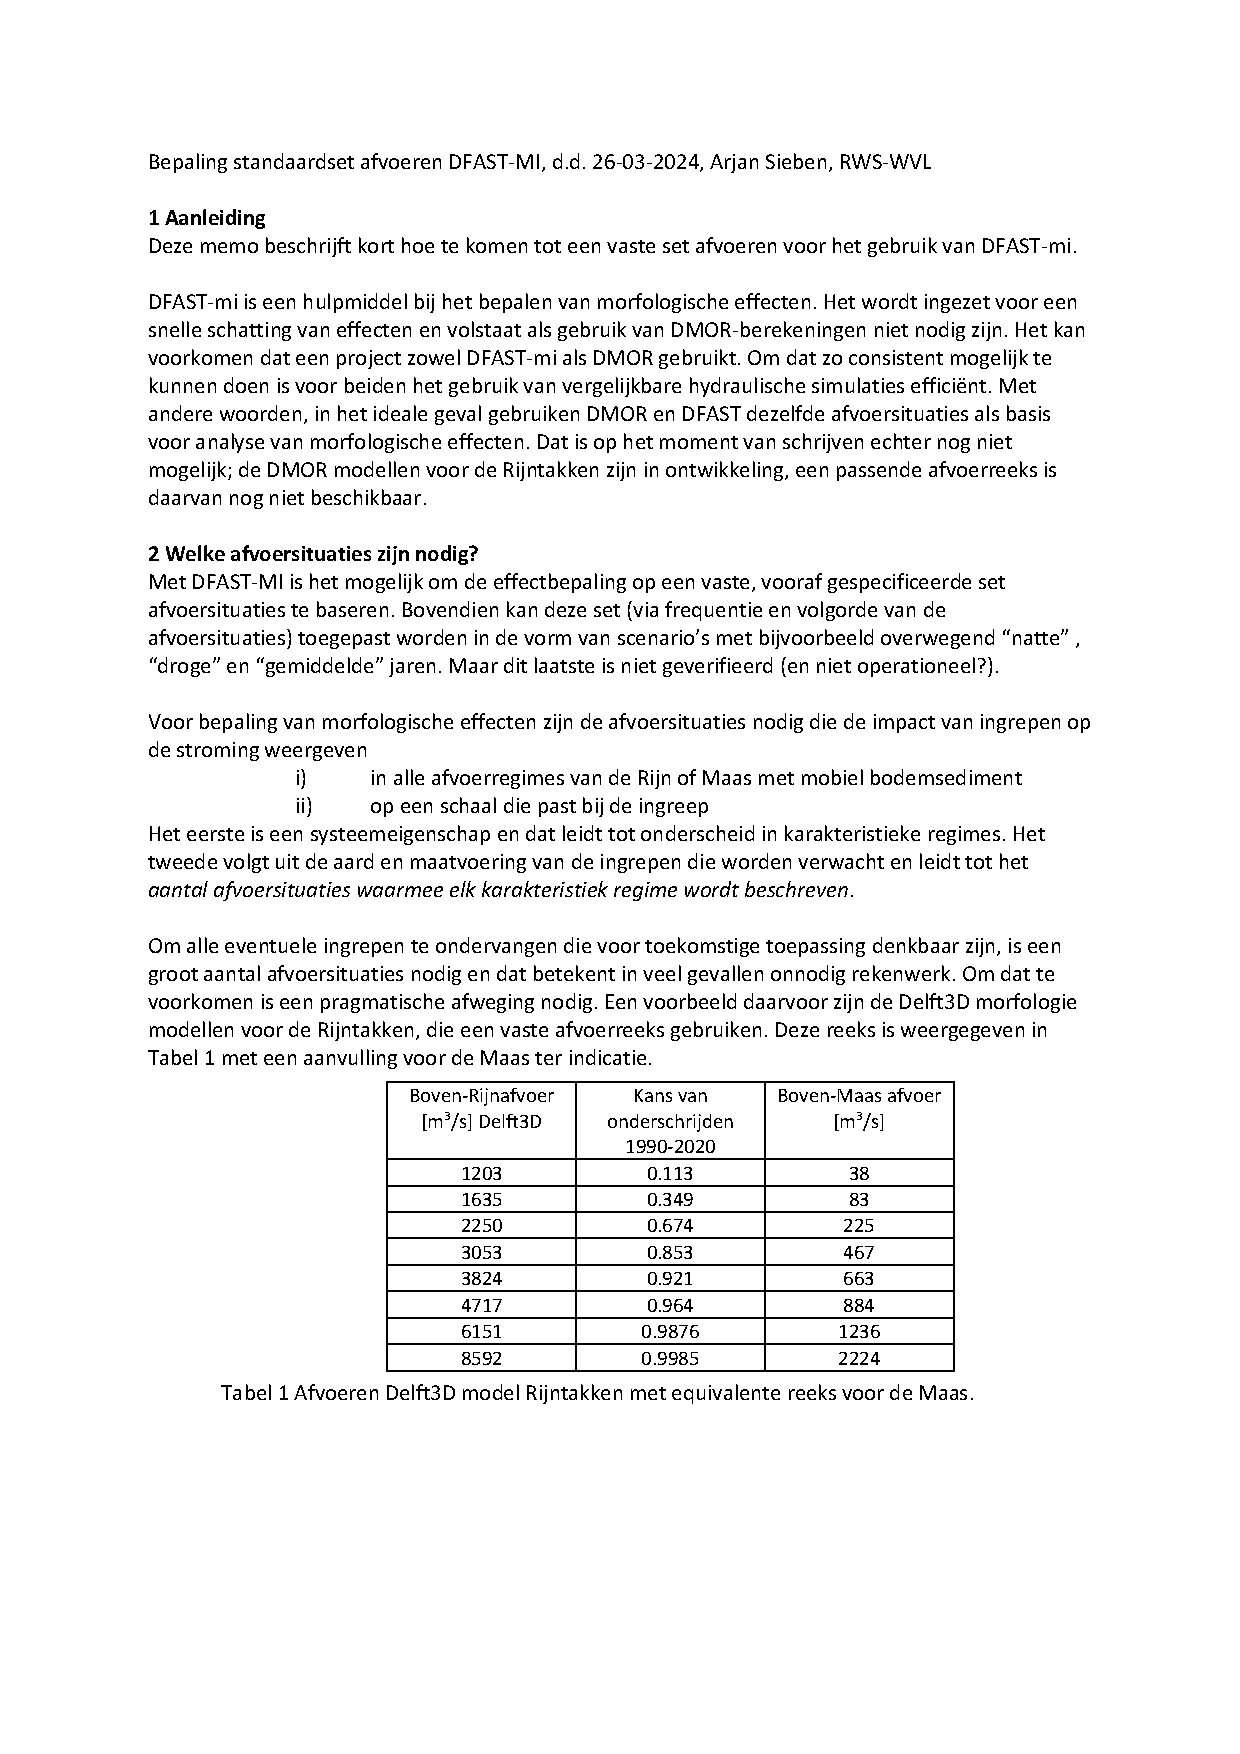
\includepdf[pages=-, offset=72 -70, frame=true, scale=0.9]{figures/afvoerblokken plus uitbreiding voortplantingssnelheden.pdf}
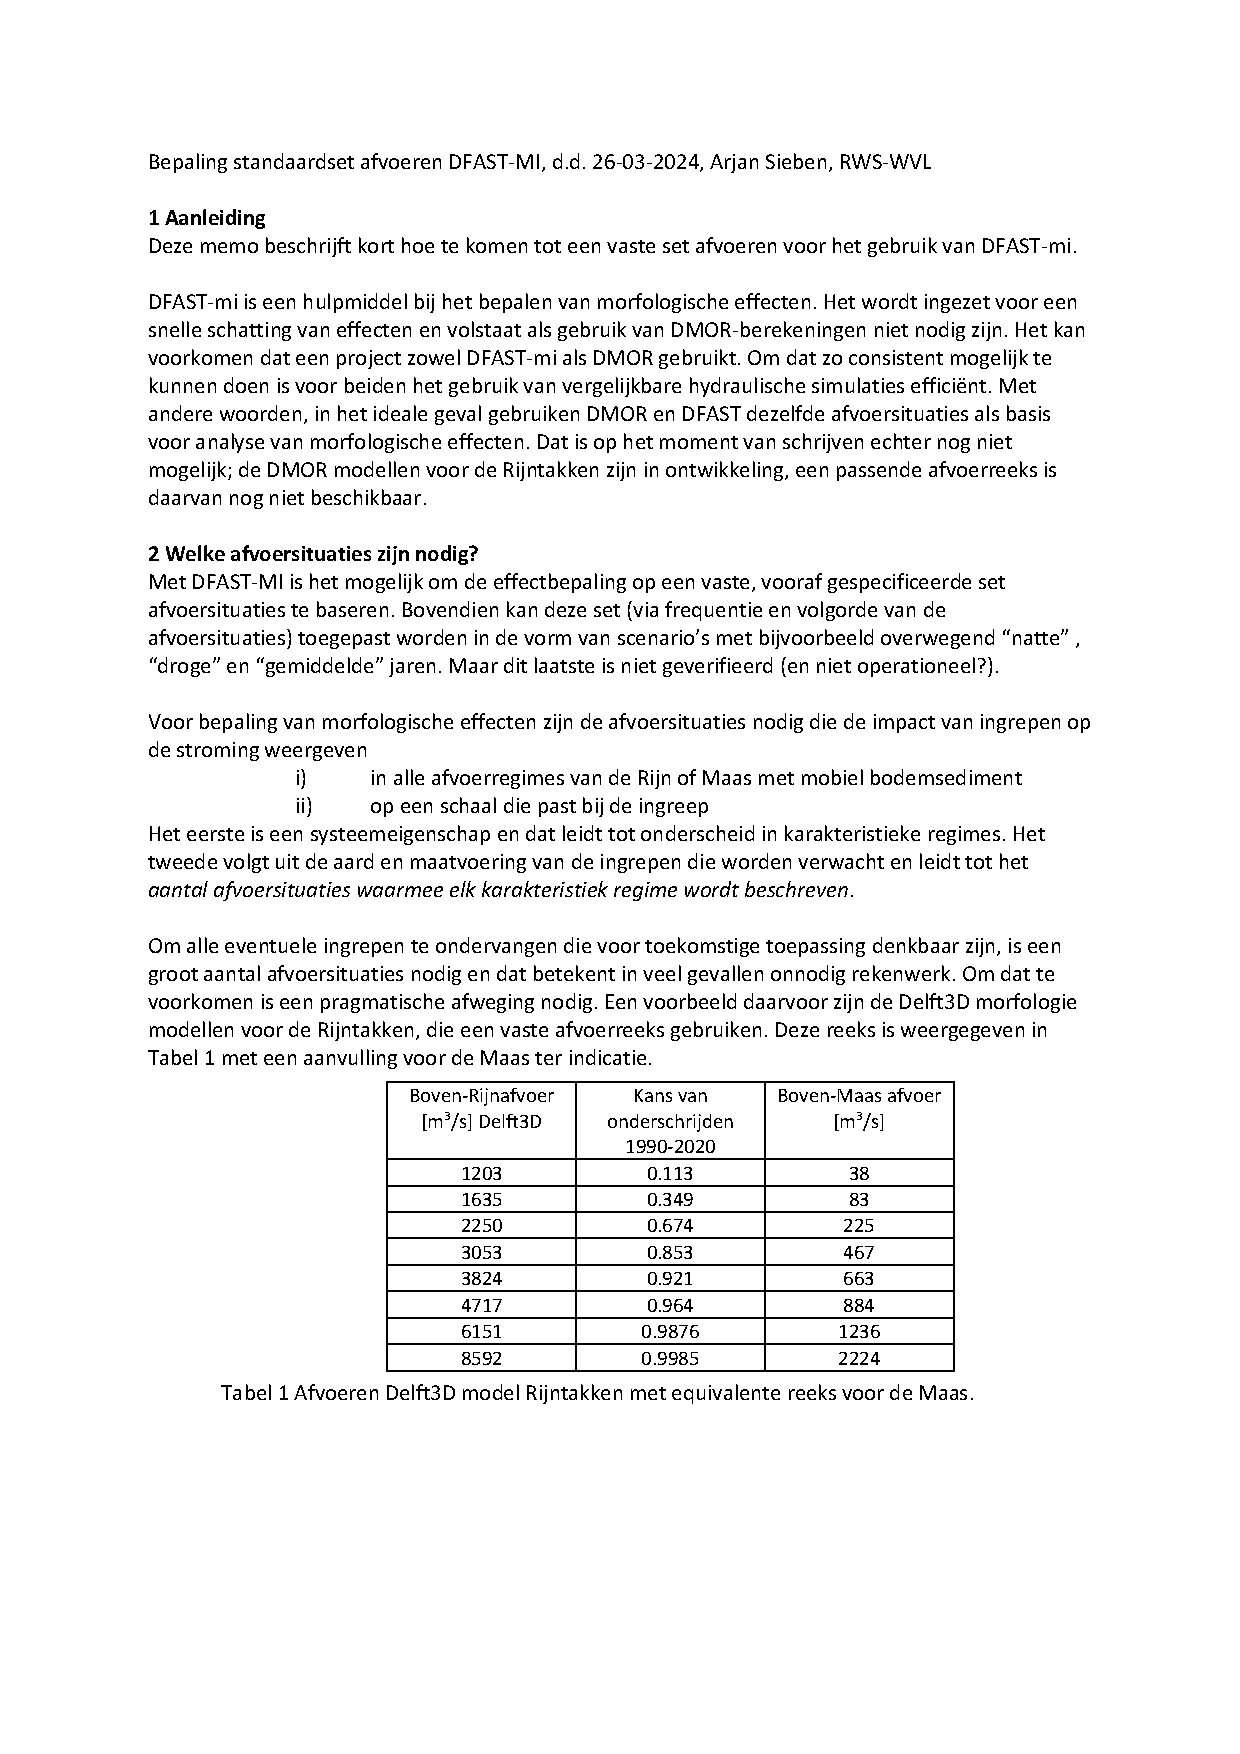
\includepdf[pages=1, offset=-72 -70, frame=true, scale=0.9]{figures/afvoerblokken plus uitbreiding voortplantingssnelheden.pdf}
\includepdf[pages=2, offset=72 -70, frame=true, scale=0.9]{figures/afvoerblokken plus uitbreiding voortplantingssnelheden.pdf}
\includepdf[pages=3, offset=-72 -70, frame=true, scale=0.9]{figures/afvoerblokken plus uitbreiding voortplantingssnelheden.pdf}
\includepdf[pages=4, offset=72 -70, frame=true, scale=0.9]{figures/afvoerblokken plus uitbreiding voortplantingssnelheden.pdf}
\includepdf[pages=5, offset=-72 -70, frame=true, scale=0.9]{figures/afvoerblokken plus uitbreiding voortplantingssnelheden.pdf}
\includepdf[pages=6, offset=72 -70, frame=true, scale=0.9]{figures/afvoerblokken plus uitbreiding voortplantingssnelheden.pdf}
\includepdf[pages=7, offset=-72 -70, frame=true, scale=0.9]{figures/afvoerblokken plus uitbreiding voortplantingssnelheden.pdf}
\includepdf[pages=8, offset=72 -70, frame=true, scale=0.9]{figures/afvoerblokken plus uitbreiding voortplantingssnelheden.pdf}
\includepdf[pages=9, offset=-72 -70, frame=true, scale=0.9]{figures/afvoerblokken plus uitbreiding voortplantingssnelheden.pdf}
\includepdf[pages=10, offset=72 -70, frame=true, scale=0.9]{figures/afvoerblokken plus uitbreiding voortplantingssnelheden.pdf}
\includepdf[pages=11, offset=-72 -70, frame=true, scale=0.9]{figures/afvoerblokken plus uitbreiding voortplantingssnelheden.pdf}

%\markdownInput[shiftHeadings=1]{techref.md}

\pagestyle{empty}
\cleardoublepage
\mbox{}

\includepdf[pages=2, offset=-72 -70]{cover/D-FAST-omslag-D-FAST Morphological Impact-UM.pdf} % links-rechts past precies
\end{document}
